
\documentclass{article}

\usepackage[titletoc,title]{appendix}
\usepackage{charter}
\usepackage{color}
\usepackage{eurosym}                         % Euro symbol
\usepackage[english]{babel}                   % English language/hyphenation
\usepackage{fancyhdr}
\usepackage{float} %For exact figure positioning
\usepackage[top=2cm, bottom=4cm]{geometry}
\usepackage{graphicx}                 % Enable pdflatex
\usepackage{hyperref}
%\usepackage{fix-cm}                         % Custom fontsizes
%\usepackage[margin=3.0cm]{geometry}
\usepackage{lastpage} % number of last page
\usepackage[protrusion=true,expansion=true]{microtype}        % Better typography

\usepackage{pifont}% http://ctan.org/pkg/pifont
\usepackage{rotating}
\usepackage[table]{xcolor}
\definecolor{ForestGreen}{RGB}{34,139,34}

\rowcolors{2}{gray!25}{white}


\hypersetup{
    colorlinks,
    citecolor=black,
    filecolor=black,
    linkcolor=black,
    urlcolor=black
}

% Definition of \maketitle
\makeatletter
\def\@maketitle{
\begin{center}
 FOSDEM AV Manual\\
{\Large  \@author}\\[4ex]
\@date\\[8ex]
 
\includegraphics[width = 80mm]{logo-gear}\\

\medskip
\noindent {\Huge \bfseries \sffamily \@title }\\[4ex]
\end{center}}
\makeatother

\setcounter{tocdepth}{4}
\setcounter{secnumdepth}{4}

\title{FOSDEM AV Manual}
\author{FOSDEM Video}
\setlength{\headheight}{44pt}

\newsavebox{\LFOSDEM}
\sbox{\LFOSDEM}{
  \mbox{
    \raisebox{0pt}[4em][0pt]{
      
\includegraphics[height=3em]{logo-gear}
    }
  }
  \parbox[b]{7cm}{
    \small{
      FOSDEM AV Manual\newline
      Version: \today{}
    }
  }
}

\newsavebox{\RFOSDEM}
\sbox{\RFOSDEM}{
  \parbox[b]{4.7cm}{
    \small{
    }
  }
}

\pagestyle{fancy}
\fancyhf{}
\rhead{\usebox{\RFOSDEM}}
\lhead{\usebox{\LFOSDEM}}
\lfoot{Version: \today}
\rfoot{Page \thepage\ of \pageref{LastPage}}


\begin{document}

\maketitle \thispagestyle{empty}
\newpage

\tableofcontents
\newpage

\section{People}
Video is a big task, so there are many people working together to make it all happen. Here's all the teams:

\subsection{AW, H, K, U and J teams}
You should be a team of at least three per building: AW, H, K and U respectively. J (probably) has a dedicated knowledgeable volunteer.

Coordination with video operations control (VOC) happens through Matrix in \#video:fosdem.org, walkies. The chat is web accessible through https://chat.fosdem.org/\#/room/\#fosdem-video:fosdem.org .

Your tasks before the conference starts:
\begin{itemize}
  \item (Friday) take the equipment to the rooms in your building
  \item (Friday) work from the biggest to the smallest room
  \item (Friday) do basic setup: cam, sound, plug in cables, basic audio checks with microphones, ... See below for details.
  \item (days of the conference) ensure the rooms are ready before the first talk starts
\end{itemize}

During the day, you'll have a fixed spot in the building. The below spots should also appear in https://nav.fosdem.org .
\begin{itemize}
  \item AW: corner between AW1.117 and AW1.121, or oneo of the top rooms (TBD)
  \item K: NOC (K.1110)
  \item H: room H.2111
  \item U: room UB4.228
\end{itemize}

Your job during the conference, with the backup from the VOC team, is to do the following in your building:
\begin{itemize}
  \item monitor video and update scene if necessary. See the ``Monitoring and control of video streams'' section for more details;
  \item assist speakers and respond to problem reports in the building;
  \item proactively fix problems with video. In some rooms, this includes preventatively replacing batteries!
\end{itemize}


\subsection{Video operations control or VOC}
You are in the NOC in the K building, with ssh access to all video machines: video laptops in the rooms, vocto machines near VOC, streaming backends and frontends, and the web pages showing the videos to our visitors.

Your job is to constantly monitor all the equipment and streams for problems, and to arrange fixes for any that occur. You have visual monitoring of all audio streams.

Do not run out to fix problems yourselves. Delegate to the per building teams. Maintaining contact between everyone is your main priority.

For more details on the monitoring, see ``Monitoring and control of video streams''.


\subsection{In the devroom}
If you are volunteering for video inside a devroom, please:
\begin{itemize}
  \item stay near the video equipment, keeping it safe (from people tripping over cables for example!)
  \item make sure the camera is aimed at the speaker
  \item monitor the devroom video/audio feeds (headphones!) for problems
  \item signal problems to VOC via matrix
\end{itemize}

Please do \emph{NOT} disconnect or turn off any equipment yourself. That is the task of the per building team only.

\section{Monitoring and control of video streams}

There should be the following monitoring available:

\begin{itemize}
  \item Page with video previews of camera, slides and mix streams, with sound leves. It can show all rooms, or a single building.\\ This is the main tool and is available at https://control.video.fosdem.org/showbuilding.php;
  \item Grafana with audio levels of the camera's input, for all rooms and selectable for a set of rooms;
  \item Ability to stream every box's stream to check for issues in video or audio - this usually an \texttt{mpv} invocation;
  \item Control interface for the video mix, to select the scene to be shown;
  \item (TBD) Host-level monitoring for all involved infrastructure, to see network outages and such.
\end{itemize}

Access to those systems is provided on Friday. Every per-building team should have a way to see the monitoring well enough, either via the in-room beamer, or some spare large screen.



\section{Rooms}
We have 28 rooms: 12 small, 14 large and 2 extra large rooms. Each type of room has a different audio/video setup.
\begin{itemize}
  \item AW: AW1120 (S), AW1121 (S)
  \item K: K1105 (XXL), K3201 (S), K3401 (S), K4201 (S), K4401 (S), K4601 (S)
  \item H: H1301 (L), H1302 (L), H1308 (L), H1309 (L), H2213 (S), H2214 (S), H2215 (L)
  \item UA: UA2214 (L), UA2118(L), UA2220 (L), UB2147 (S), UB2252A (L)
  \item UB4: UB4132 (S), UB4136 (S), UB5132 (L), UB5230 (L, spare)
  \item UD: UD2120 (L), UD2208 (L), UD2218A (L)
  \item J: Janson (XXL)
\end{itemize}

Your team's flight case comes with a printed map of where the video gear goes in your rooms. Audio and power cabling should be arranged loose on the floor, or taped down after coordination with the network team! When taping down XLR cables, please provide sufficient slack for getting up to the camera. It is about 2m above ground level!

\subsection{Small rooms}
These have a projector and a tie pin microphone for the speaker. Audience questions are picked up by the camera's internal microphone.

The connections there are as follows:

\begin{itemize}
  \item USB cable from laptop to video-box (2 laptops/boxes)
  \item Network cable (video VLAN) to the presenter box (any port)
  \item Network cable form the presenter to camera box (any port, one on each box)
  \item Laptops, camera to AC power
  \item XLR cable from the microphone receiver to channel 1 (LEFT) of the camera
  \item USB powerbank to the microphone receiver
  \item HDMI from the camera to the HDMI port of the video box
  \item VGA cable from the presenter box left HDMI port to the beamer in the room (if the beamer is VGA; use the provided adapter)
  \item HDMI cable from the presenter box to the beamer in the room (if the beamer is HDMI)
  \item HDMI cable from the speaker's laptop to the right HDMI port of the presenter box
\end{itemize}
\subsubsection{Cabling diagram}
\begin{figure}[H]
  \begin{sideways}
  \centering
  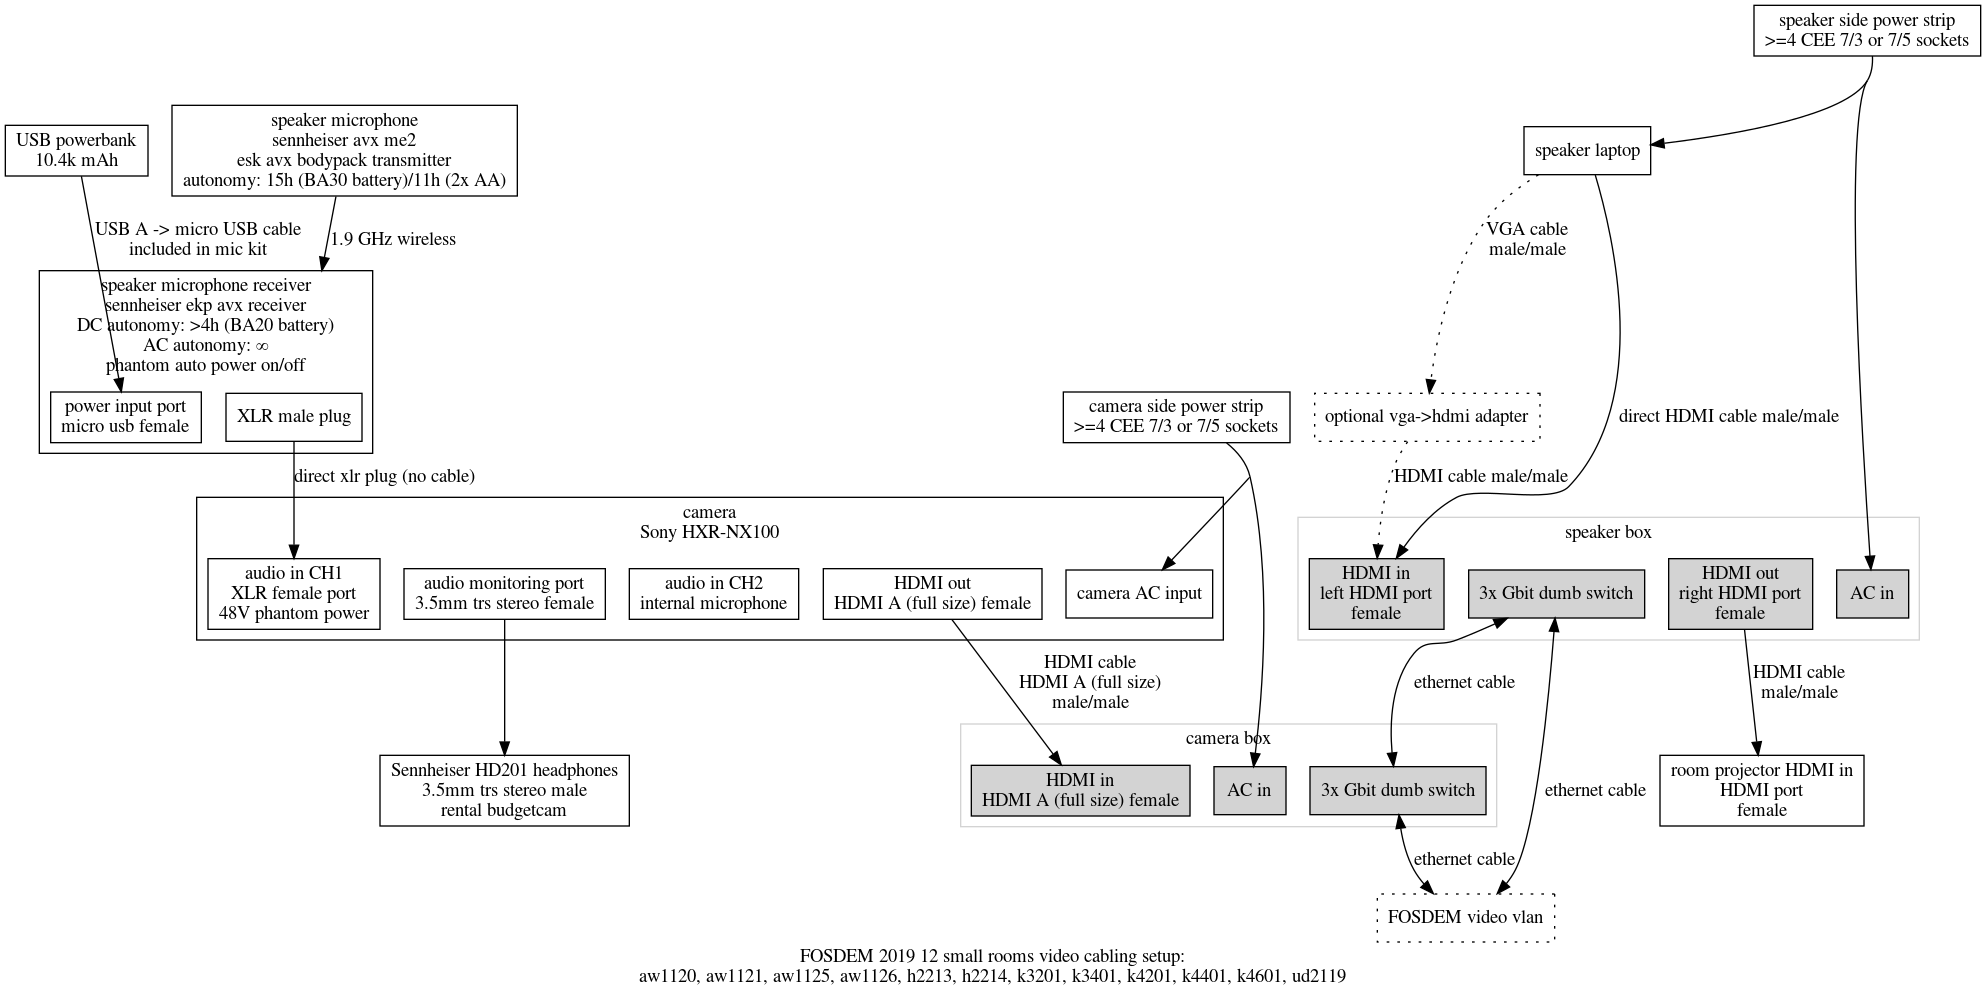
\includegraphics[width = 200mm]{../../graph/cabling_small_rooms.png}
  \end{sideways}
\end{figure}

\subsection{Large rooms}
These have a projector, a tie pin mic for the speaker and an audience microphone. They use the Sony HXR-NX100 camera. For the rooms that don't have a PA, there's also a dedicated speaker.

The connections there are as follows:

\begin{itemize}
  \item USB cable from laptop to video-box (2 laptops/boxes)
  \item Network cable (video VLAN) to the presenter box (any port)
  \item Network cable form the presenter to camera box (any port, one on each box)
  \item Laptops, camera, audio mixer to AC power
  \item Microphone receiver for the speaker microphone to channel 1 of the mixer
  \item Microphone receiver for the audience microphone to channel 2 of the mixer
  \item XLR cable from the left channel of the audio mixer to channel 1 (LEFT) of the camera
  \item XLR cable from the AUX channel of the audio mixer to the room PA or speaker
  \item USB powerbank to the microphone receivers
  \item HDMI from the camera to the HDMI port of the video box
  \item VGA cable from the presenter box left HDMI port to the beamer in the room (if the beamer is VGA; use the provided adapter)
  \item HDMI cable from the presenter box to the beamer in the room (if the beamer is HDMI)
  \item HDMI cable from the speaker's laptop to the right HDMI port of the presenter box
\end{itemize}
\subsubsection{Cabling diagram}
\begin{figure}[H]
  \begin{sideways}
  \centering
  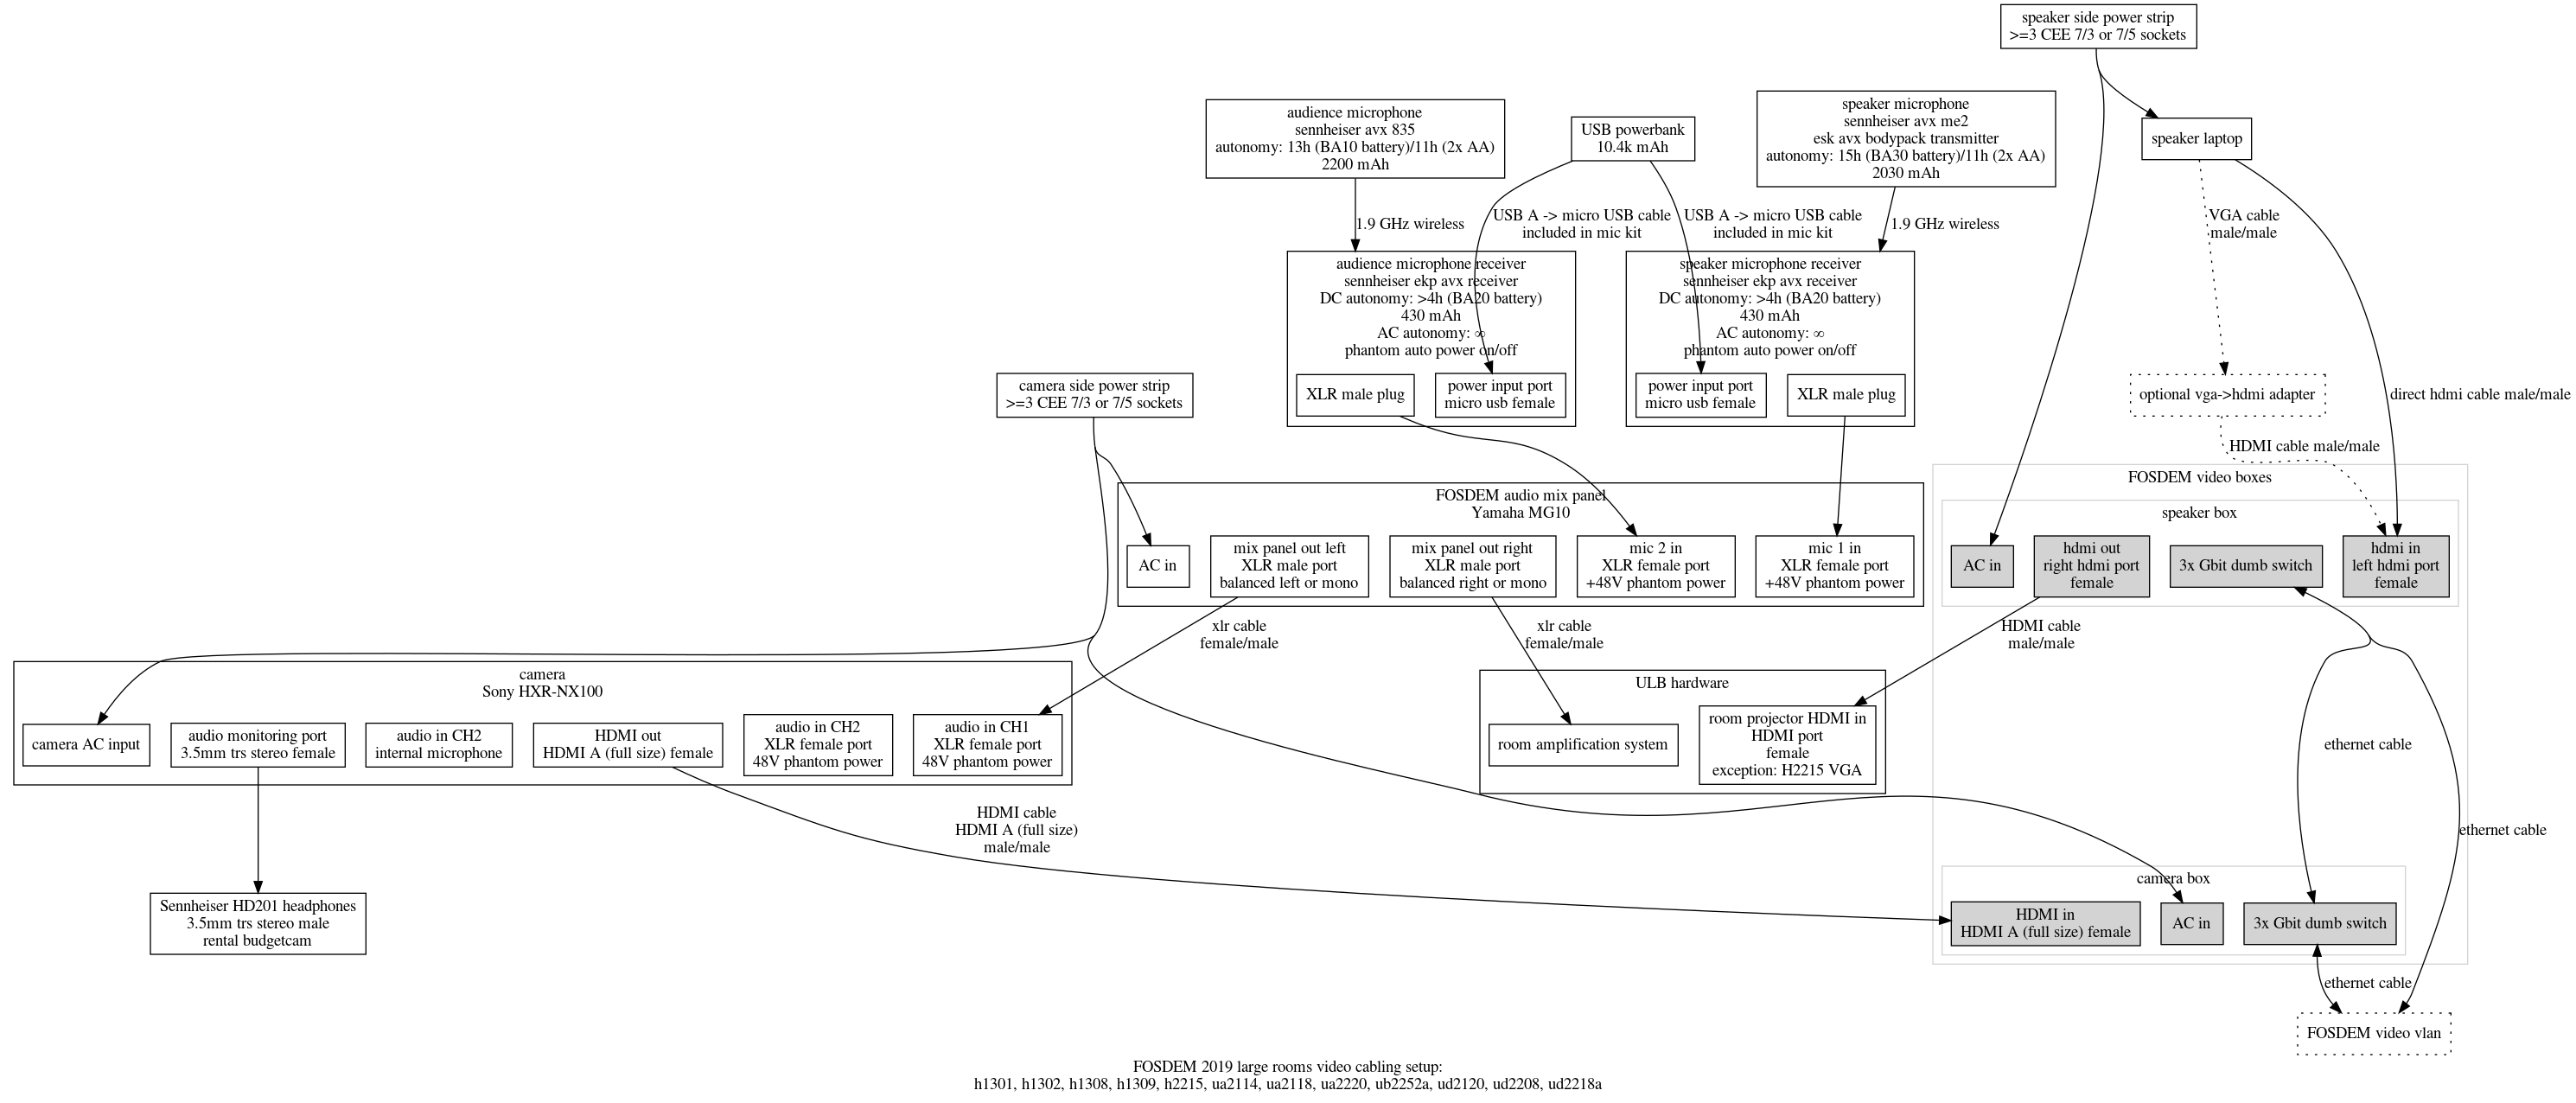
\includegraphics[width = 200mm]{../../graph/cabling_large_rooms.png}
  \end{sideways}
\end{figure}

\subsection{Extra large rooms}
These have a projector, a tie pin mic for the speaker and one or two audience microphones. They use the Sony HXR-NX100 camera.

The connections there are as follows:

\begin{itemize}
  \item USB cable from laptop to video-box (2 laptops/boxes)
  \item Network cable (video VLAN) to the presenter box (any port)
  \item Network cable form the presenter to camera box (any port, one on each box)
  \item Laptops, camera to AC power
  \item XLR cable from the left channel of the audio mixer (ULB provided) to channel 1 (LEFT) of the camera
  \item HDMI from the camera to the HDMI port of the video box
  \item VGA cable from the presenter box left HDMI port to the beamer in the room (if the beamer is VGA; use the provided adapter)
  \item HDMI cable from the presenter box to the beamer in the room (if the beamer is HDMI)
  \item HDMI cable from the speaker's laptop to the right HDMI port of the presenter box
\end{itemize}

\subsubsection{Cabling diagram}
\begin{figure}[H]
  \begin{sideways}
  \centering
  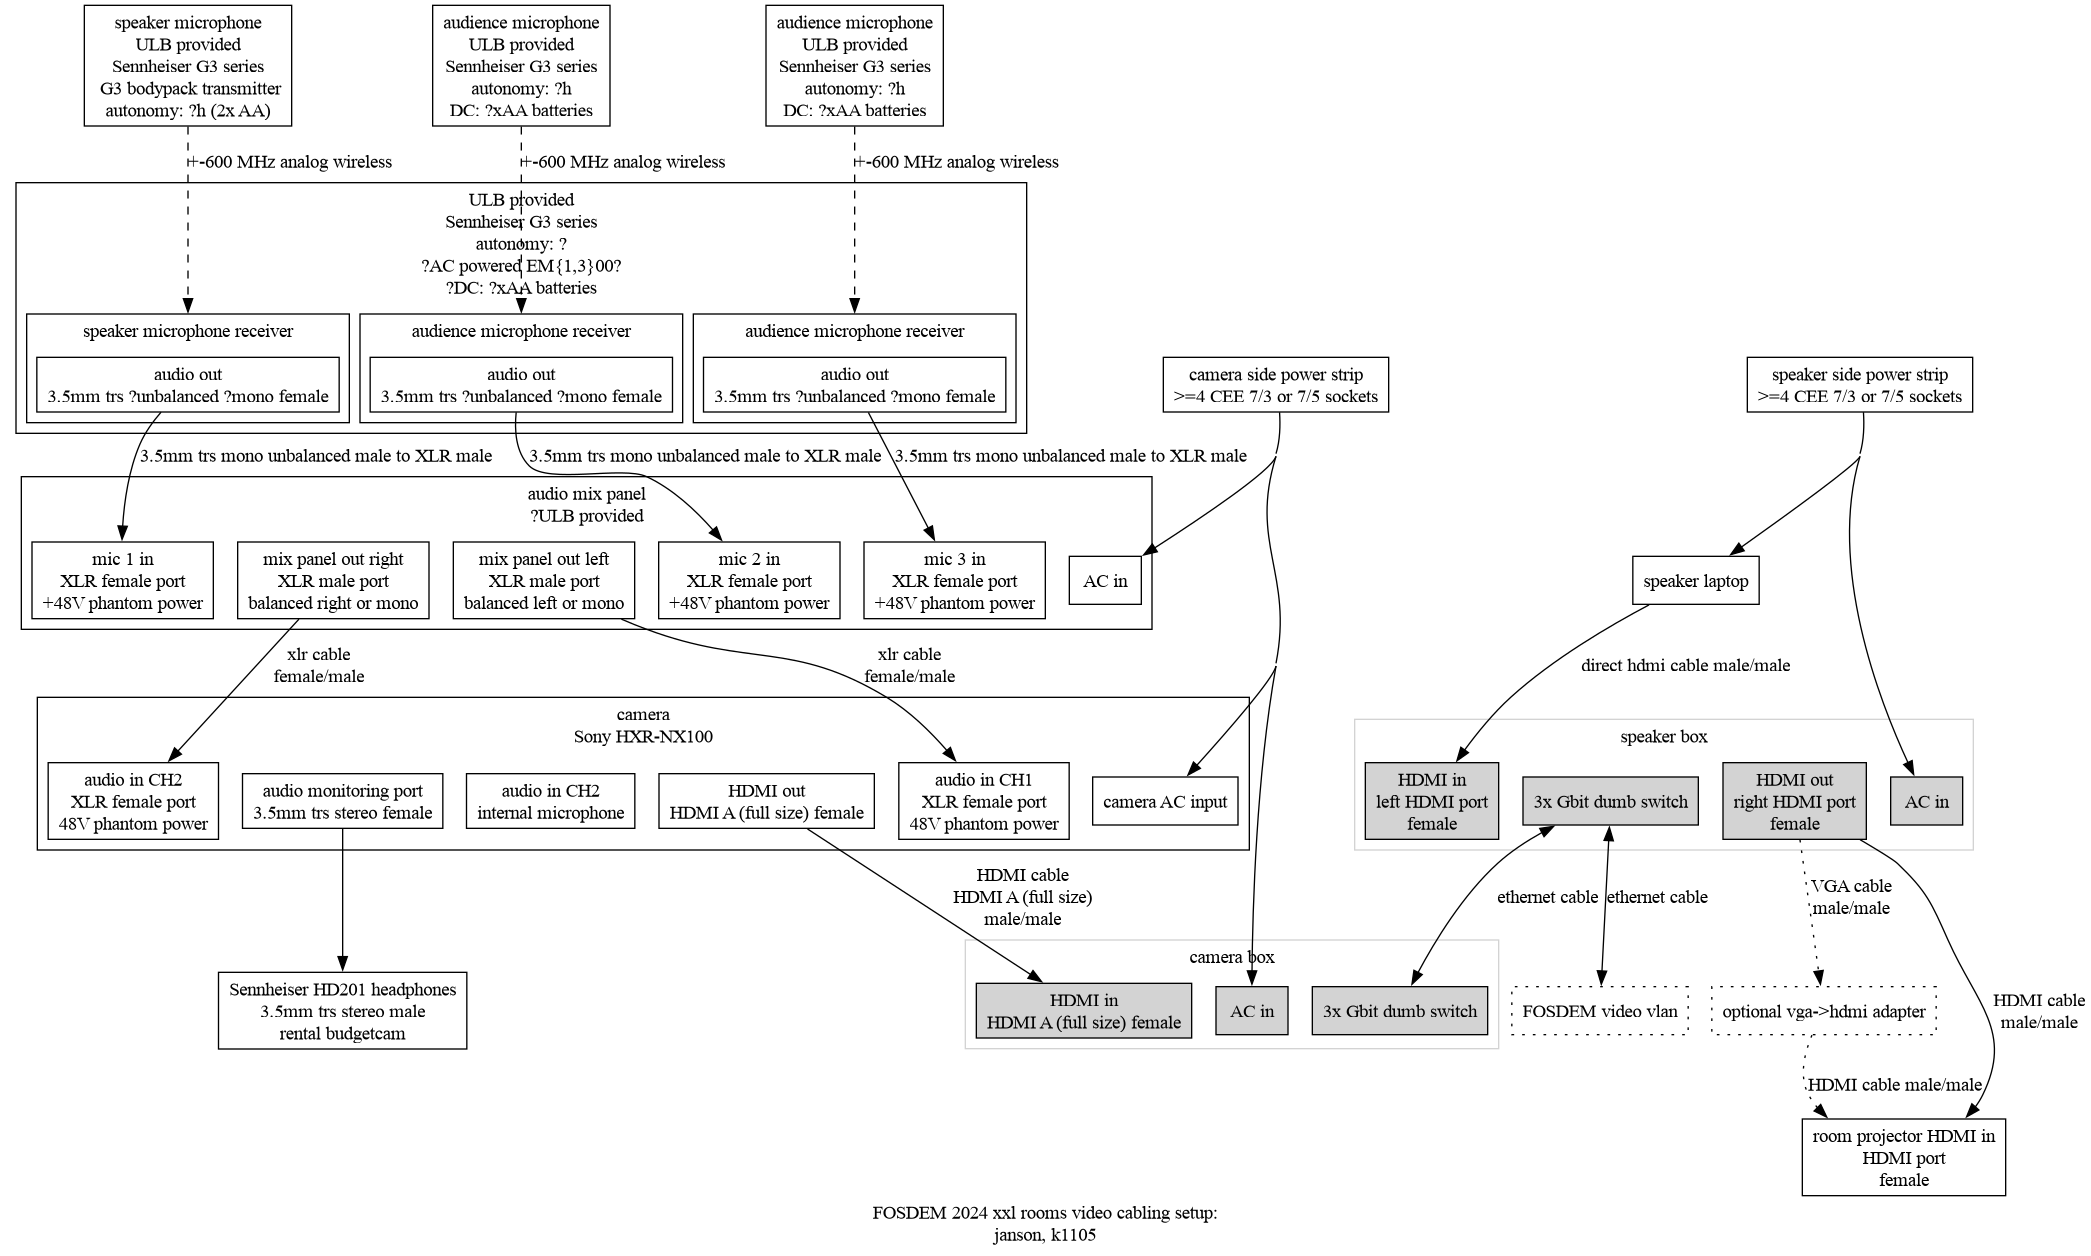
\includegraphics[width = 200mm]{../../graph/cabling_xxl_rooms.png}
  \end{sideways}
\end{figure}

\section{FOSDEM video boxes}
The FOSDEM video box and its control laptop will take care of the streaming and recording.
There is no need to operate the controls on the camera (once on and in the correct video mode, which the setup team will have done). The setup team should also have connected the following:
\begin{itemize}
  \item at least one network cable
  \item a power cable, connected to mains, with the box already turned on
  \item slides boxes (the one for the speaker) only:
    \begin{itemize}
      \item The right HDMI connection should be connected to the projector
      \item The left HDMI connection should have a loose HDMI cable, for connecting to the presenter laptop
    \end{itemize}
  \item Cam boxes only:
    \begin{itemize}
      \item An HDMI cable to the (powered on) camera
    \end{itemize}
\end{itemize}

\iffalse
The power switch is at the back, on a standard power supply:
\begin{figure}[H]
  \centering
  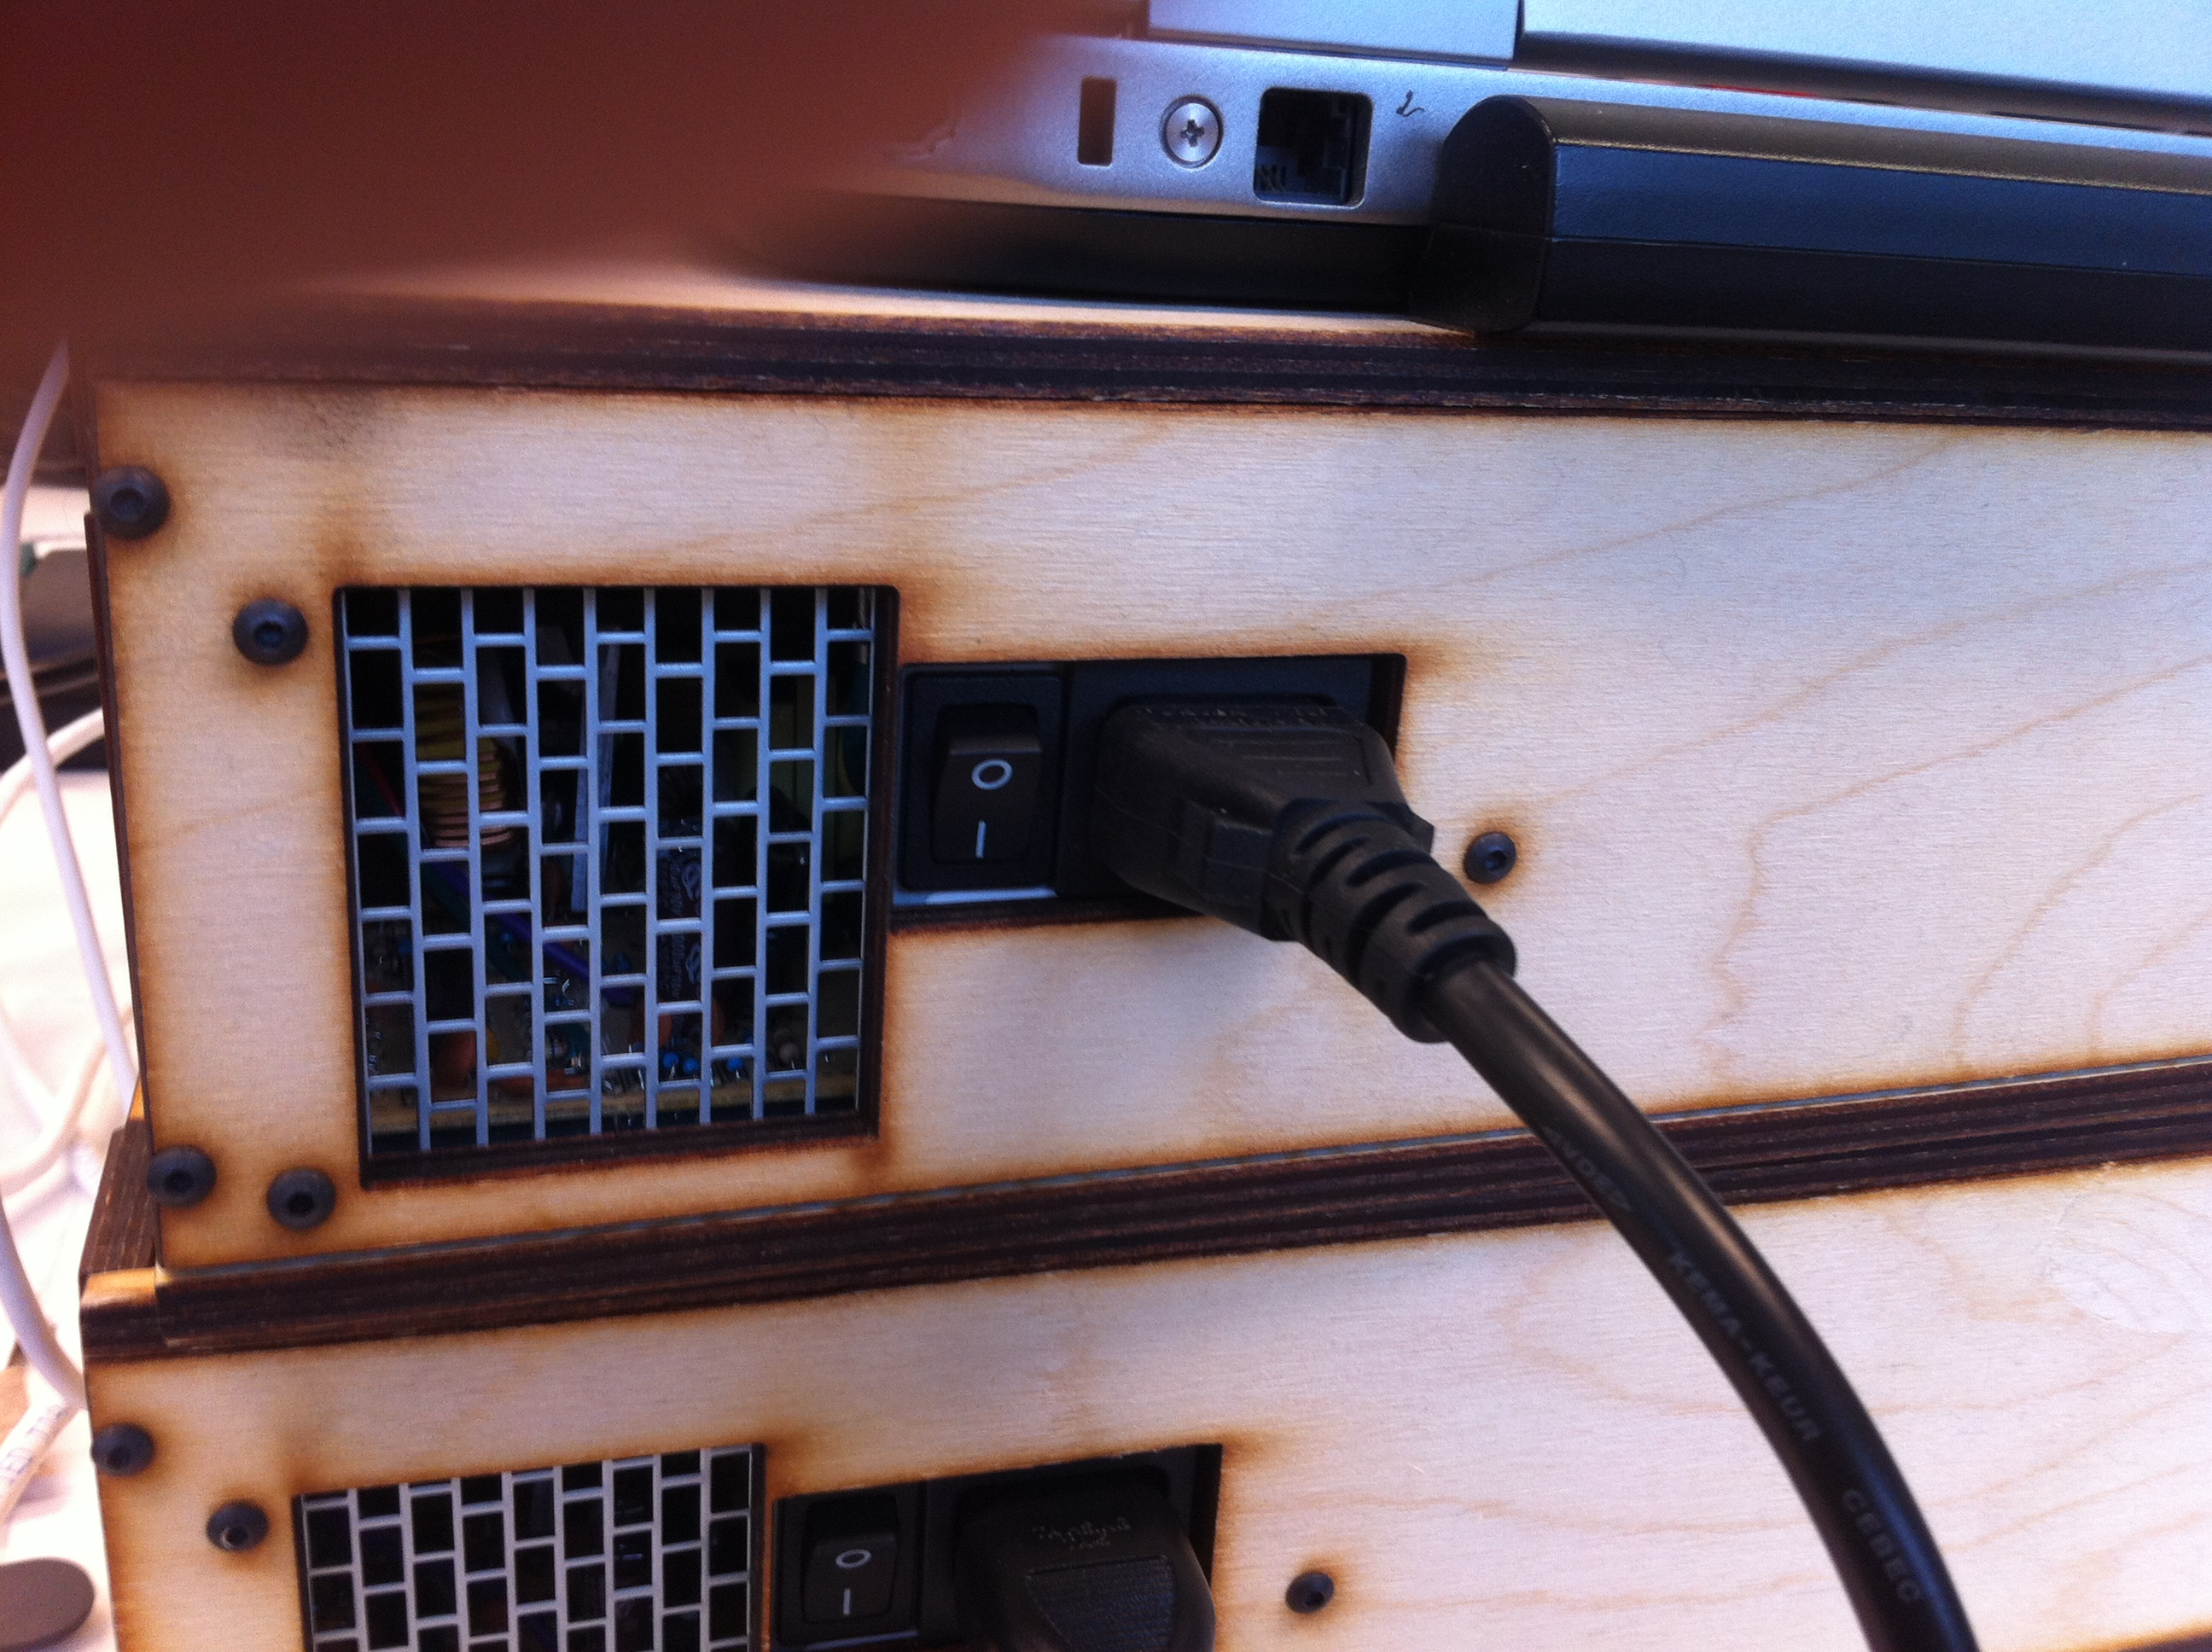
\includegraphics[width = 120mm]{videobox_psu.jpg}
\end{figure}
\fi

Order of connections and powering on does not matter, each order will work. There is no need to reboot the box after connections have changed.
Fully booting the laptop takes about a minute, and it should show a graphical interface with data on the left and video on the right.

\emph{Do not attempt to power off the box unassisted, as this may damage the integrity of the system.}
In the event of power loss or accidental unplugging, the system should stay up due to the built-in battery, we don't expect it to stay without power long enough to actually go down. If you suspect it may be malfunctioning and there is not enough diagnostic information, contact the control and monitoring team (see chapter ``During the event'' for full details). They may already be aware of the problem, but quick reporting helps cut down on reaction times.

While the box contains a network switch (all four ports are connected), \emph{do not connect your own equipment} to the box. The boxes are on a special subnet with reserved bandwidth for the video streaming, and any other equipment may compromise the quality of the broadcast.

\emph{The boxes have only HDMI input and HDMI output.}
For speakers with only VGA outputs, the per-building video team is required to ask them for their time machine license registration. Mini-DP and some other connectors might be available with the per-building team.
The HDMI signal is automatically scaled to 1080p (1920x1080) at 50Hz. Matching this on the presenter laptop is a good idea, but not a requirement.

\emph{The control laptop display will inform you of all vital information about the current status of the box.} It shows the stream video on the right with the sound levels overlayed on its top left corner, signal and its network status (connected/disconnected), the recording status (yes/no), the streaming status (yes/no) and others.

The boxes report all this information to control while their network status is good, where the control and monitoring team keeps on eye on all rooms. If something is wrong, they may send somebody your way to correct it. Please follow the instructions (if any) of video team members. Keeping an eye on the box vitals and correcting any problems you notice is encouraged.

\section{Tripod}
We use the Manfrotto MVH 502. This should hopefully be self-explanatory. Please offer feedback to VOC if that is not the case.

\clearpage

\section{Camera}
FOSDEM 2024 will use one camera model: the Sony HXR-NX100.

\subsection{Standard camera settings and quick checklist}
\begin{tabular}{| l | l |}
\hline
Resolution & 1920x1080 \\
Refresh rate & 50p \\
MIC-CHANNEL1(left) & Speaker and audience microphone \\
MIC-CHANNEL2(right) & Internal microphone \\
Power source & Cable AND Battery \\
Lens cover & Remove! \\
Camera/Tripod & Cam must be attached to tripod plate \\
\hline
\end{tabular}

\subsection{Setup for large and extra large rooms}

\subsubsection{Screw camera on mount}
Screw the camera onto the tripod. Every camera has a screw hole at the bottom that can be used for this. The plate has a distinct ``point camera in this direction'' arrow, pay attention to this. The screw can be tightened by a coin or similar object.

\begin{figure}[H]
  \centering
  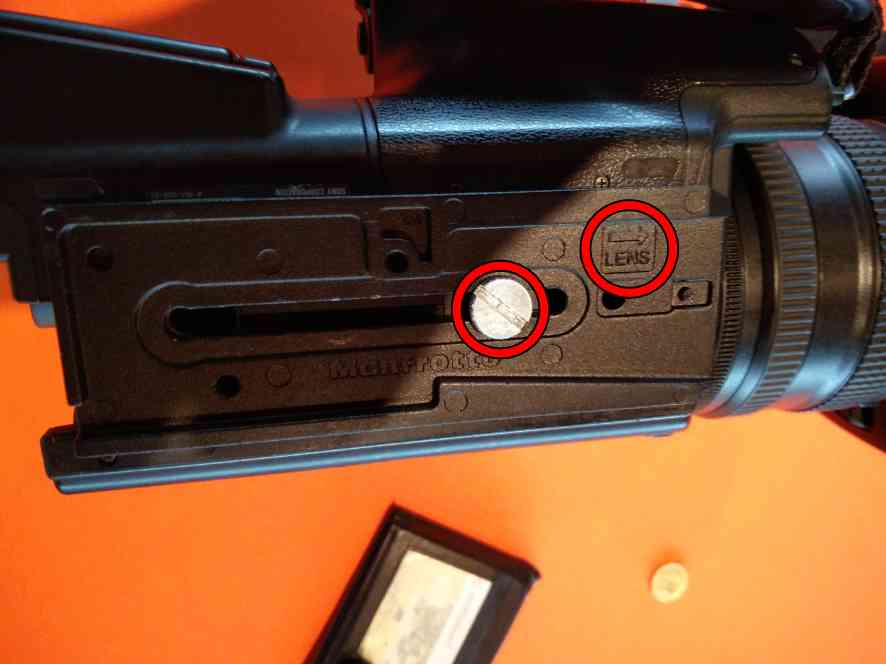
\includegraphics[width = 120mm]{Cam00.jpg}
\end{figure}

\subsubsection{Power and HDMI connectors}
First plug in the battery at the back, then plug in both the HDMI and the power cable.
Both connectors can be found next to each other to the right of the battery slot at the back.
Look at the picture if you're unsure.

Do not forget to hook up the other end of the HDMI cable to the FOSDEM Video Box and the power cable into the mains.

\begin{figure}[H]
  \centering
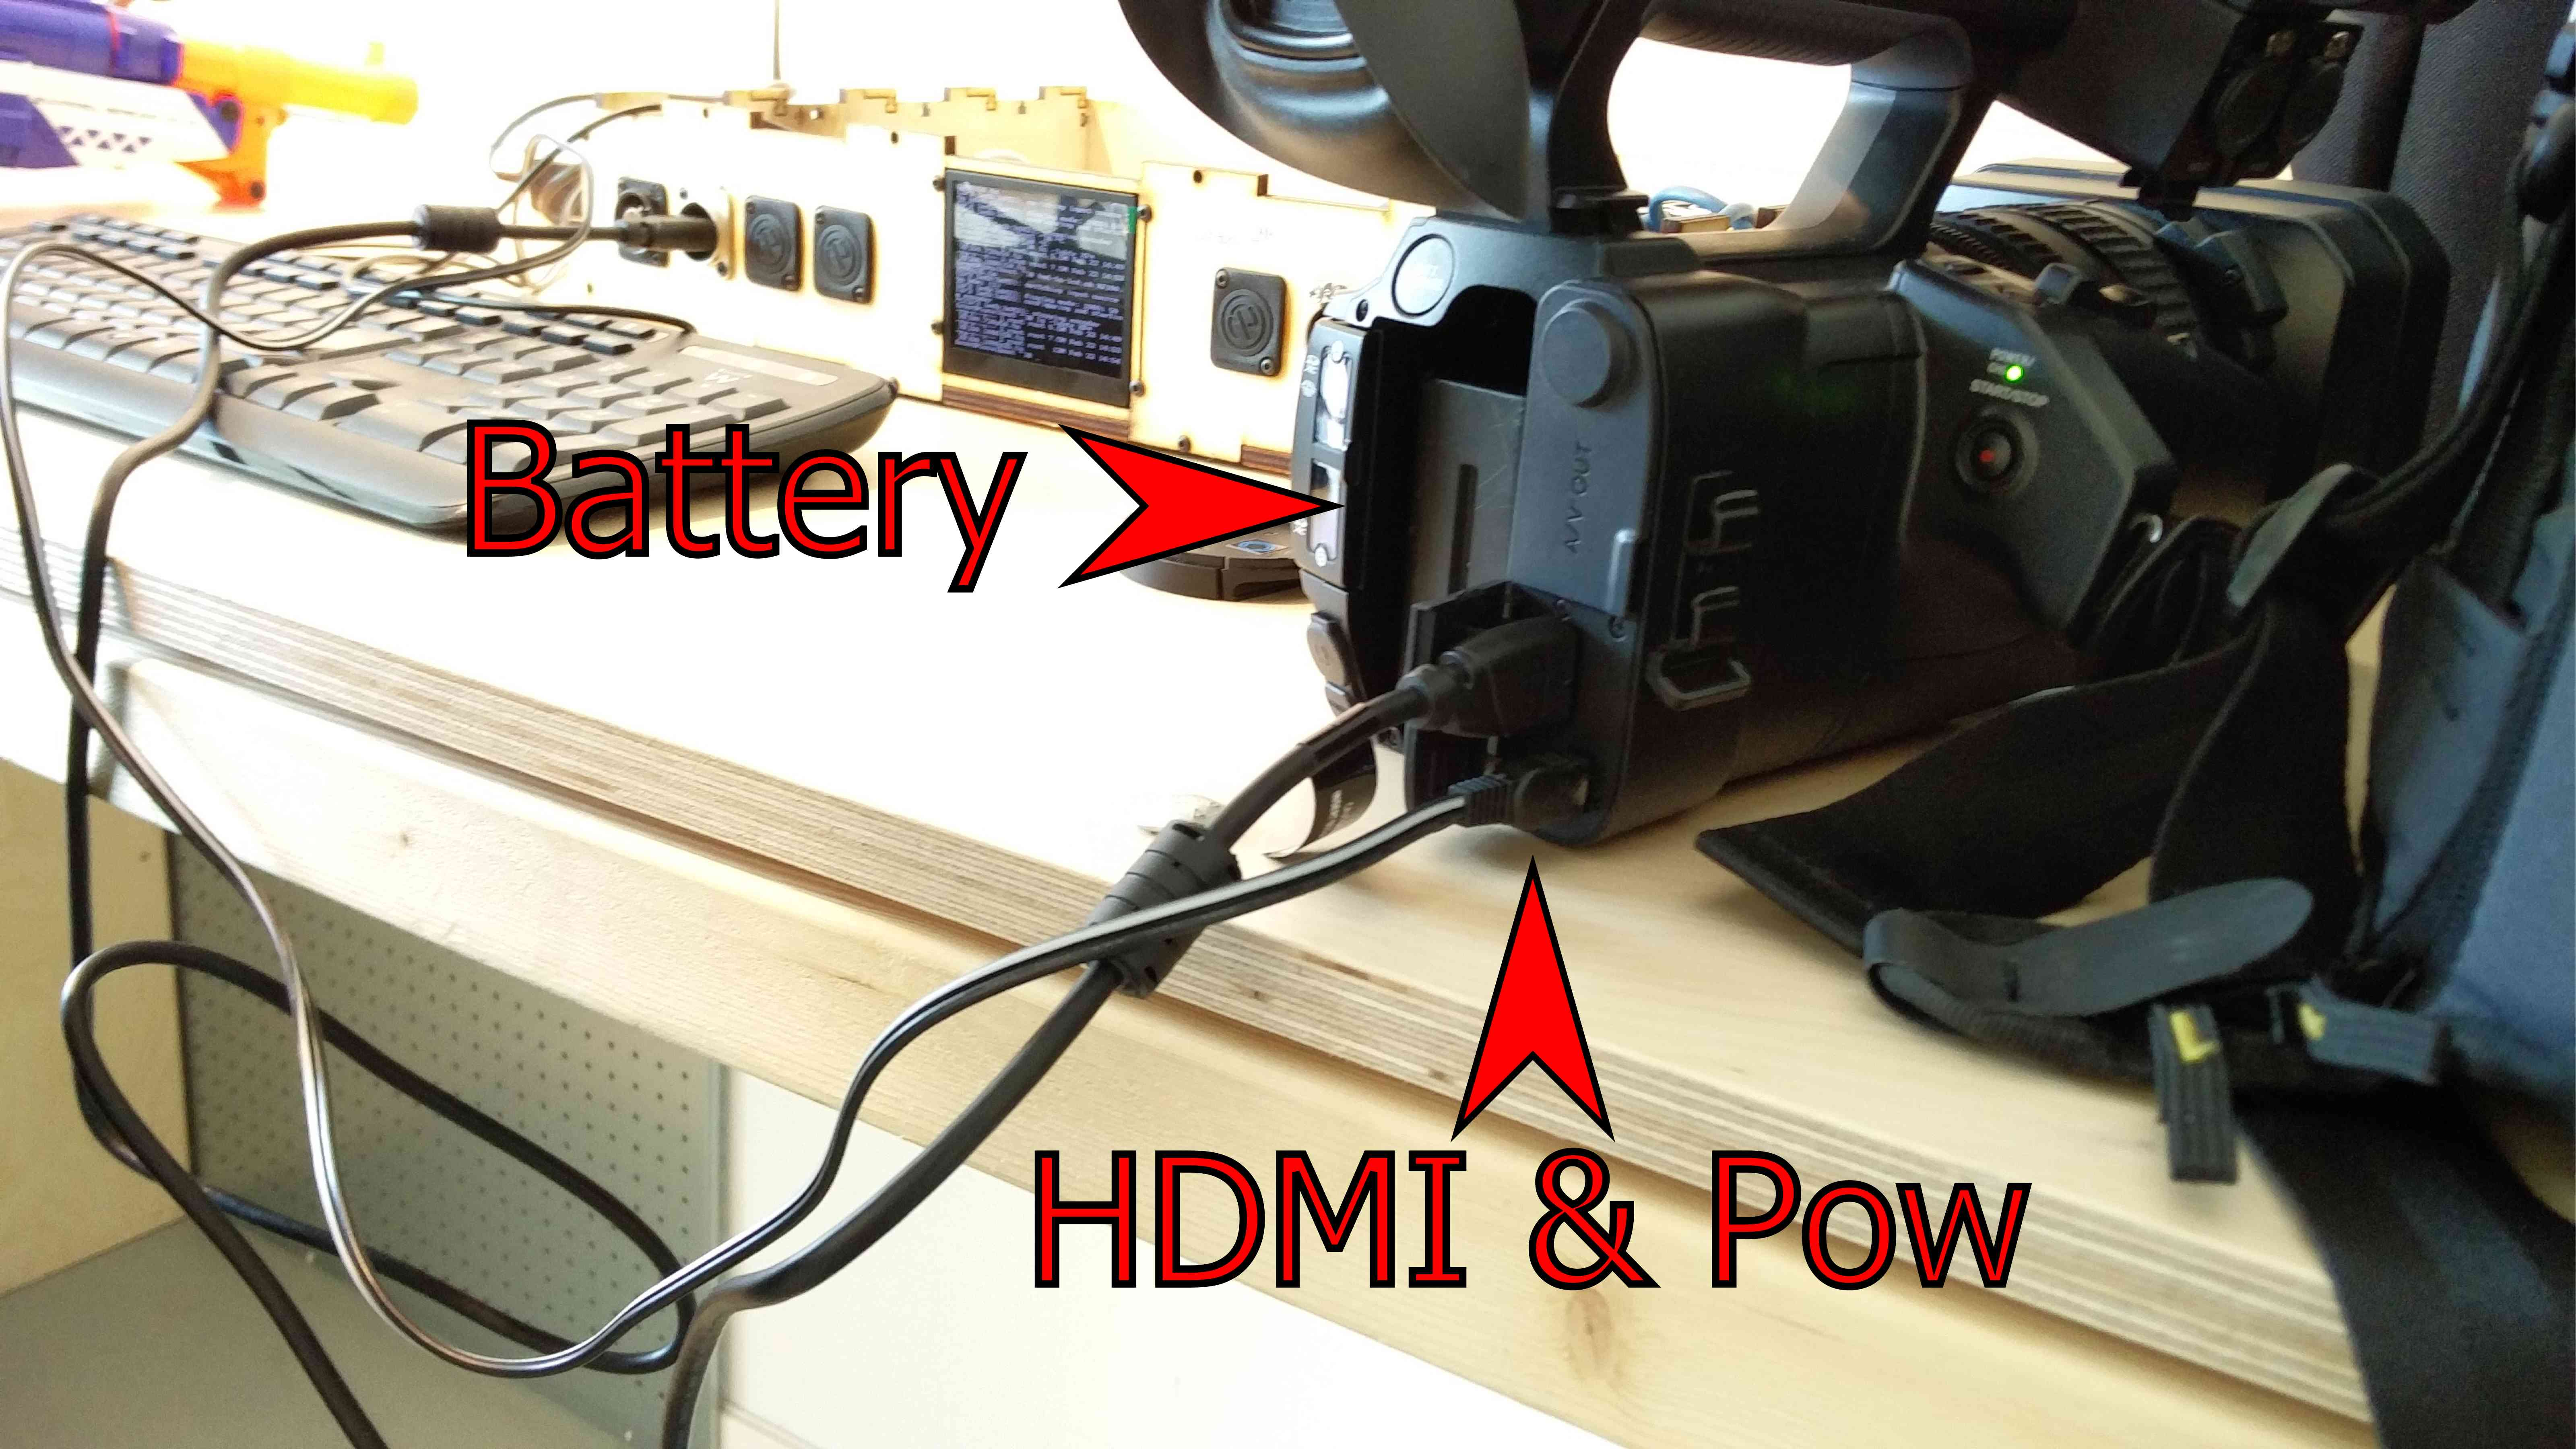
\includegraphics[width = 120mm]{Sony01.jpg}
\end{figure}

\subsubsection{Microphone}
Plug the XLR cable of the audio system into Input1.

\begin{figure}[H]
  \centering
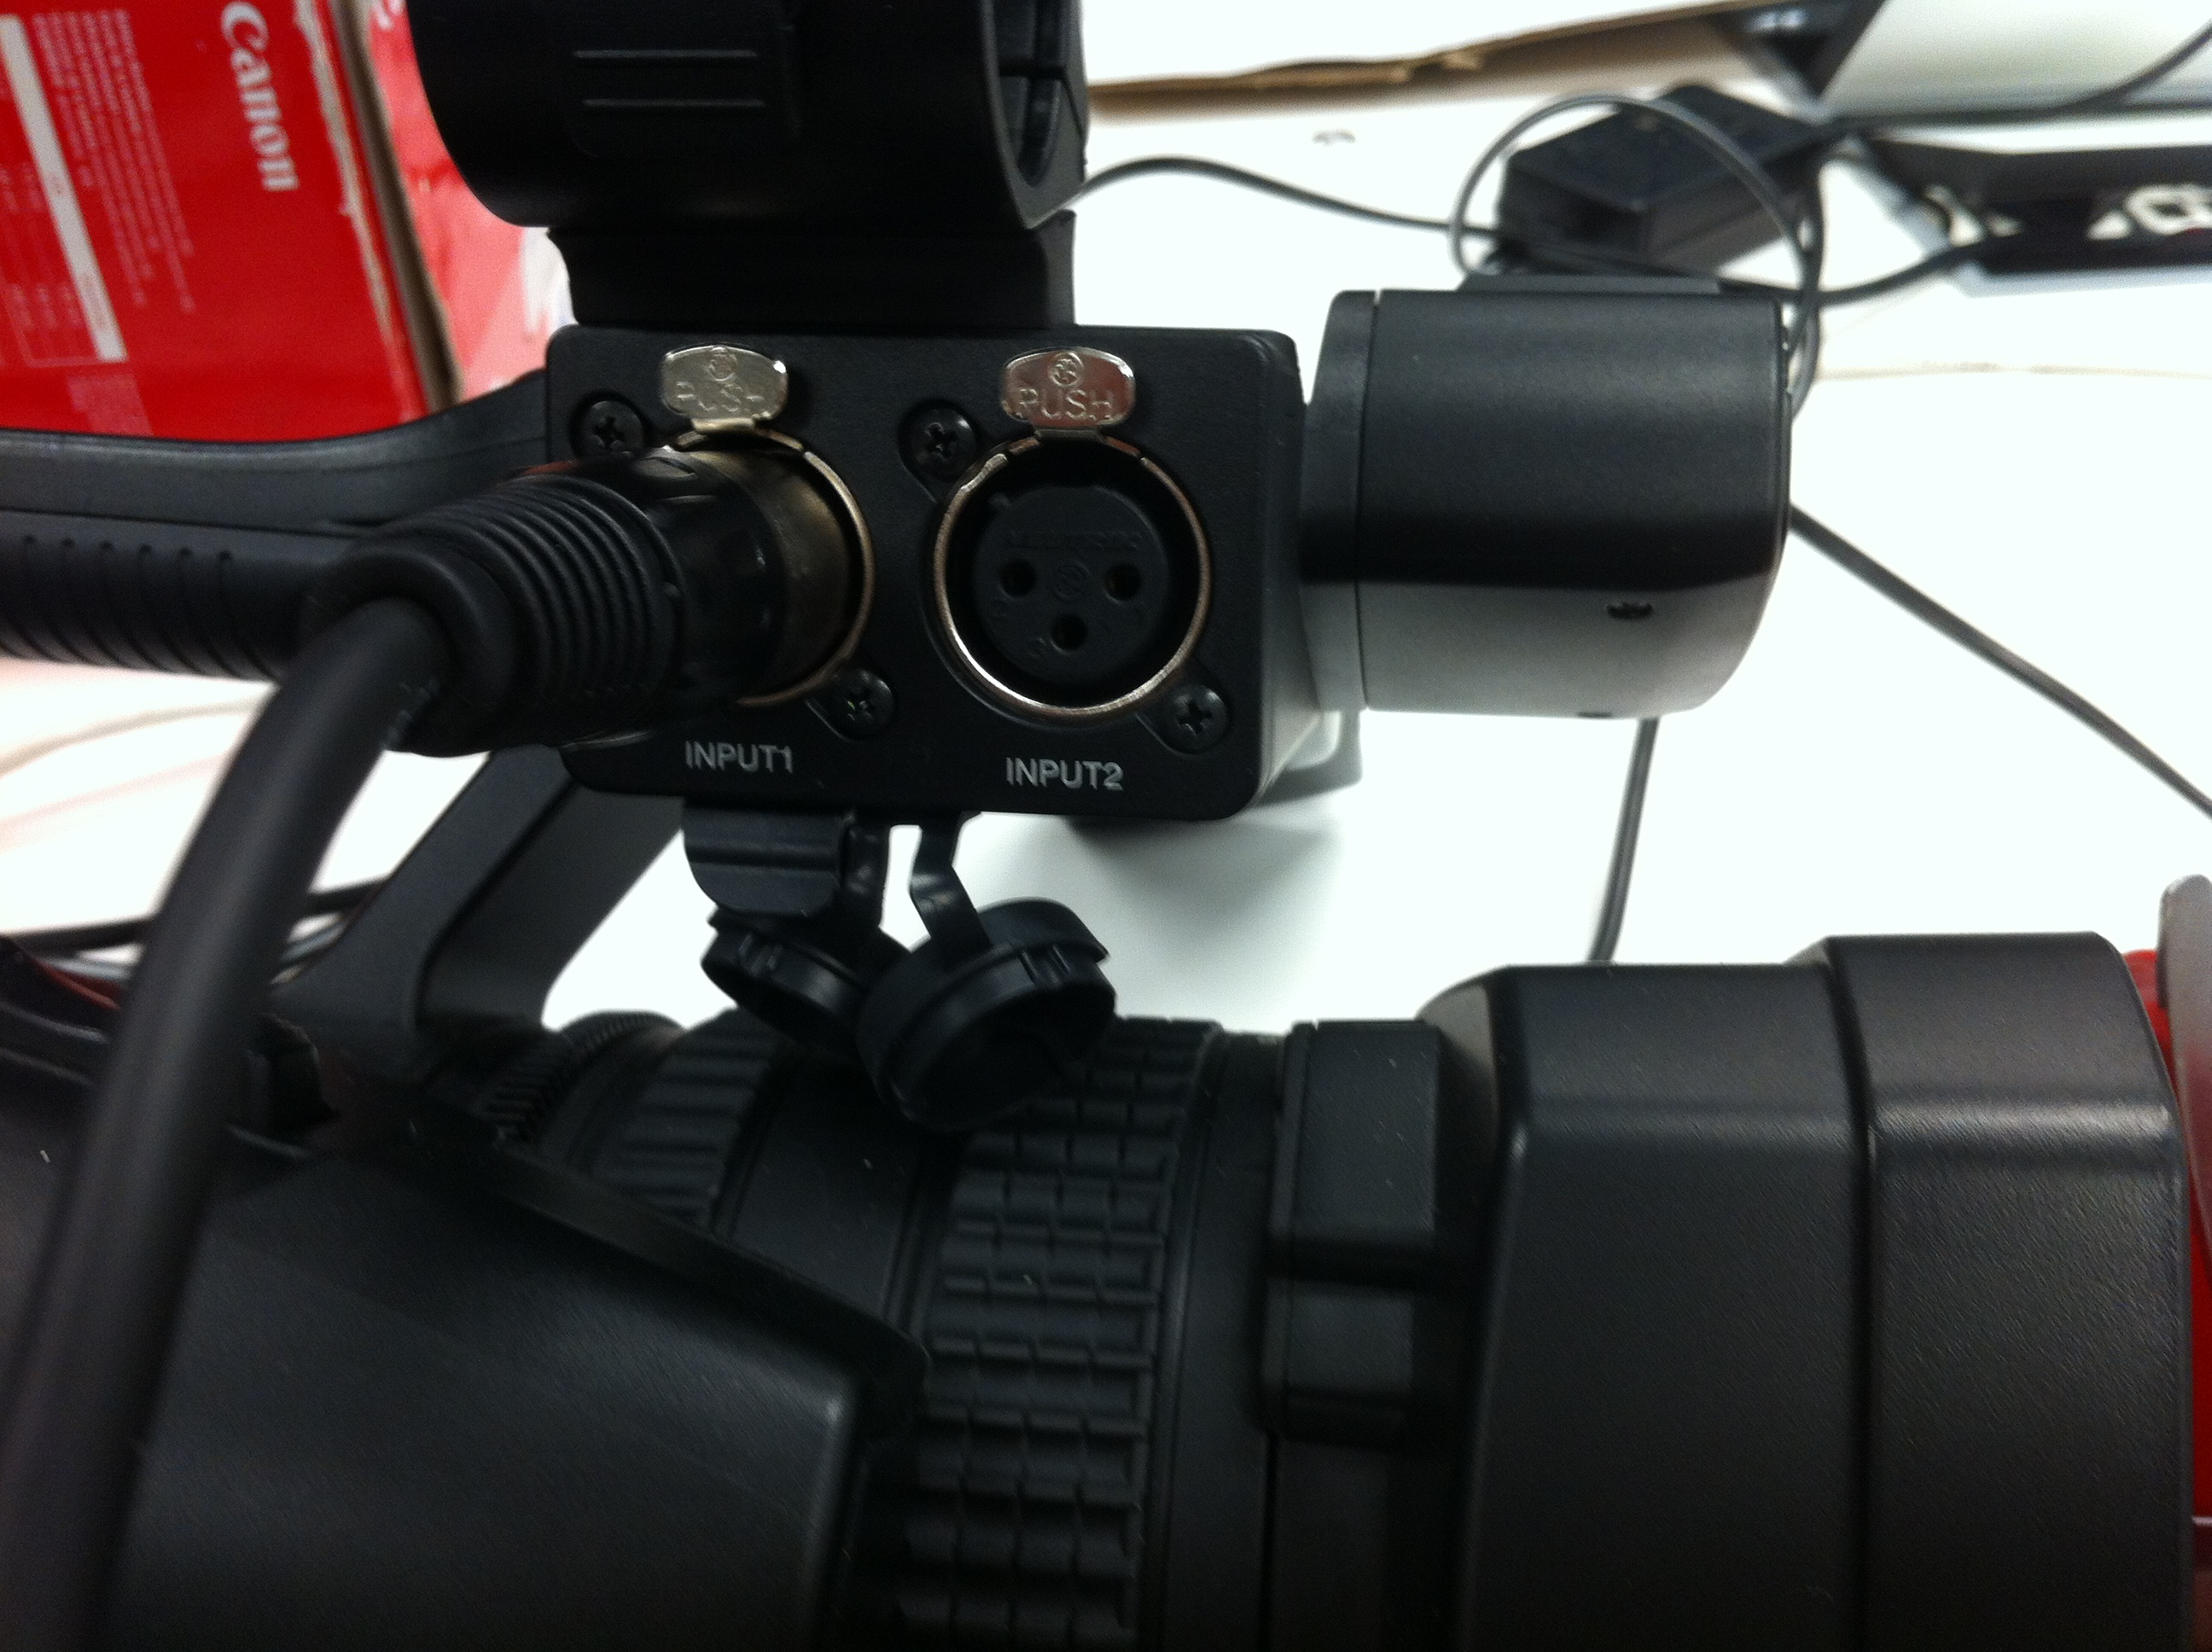
\includegraphics[width = 120mm]{sony_connect_xlr.jpg}
\end{figure}

\subsubsection{Power on}
You can find the power button on the left side of the camera (looking from behind). Look in the bottom right corner.

\begin{figure}[H]
  \centering
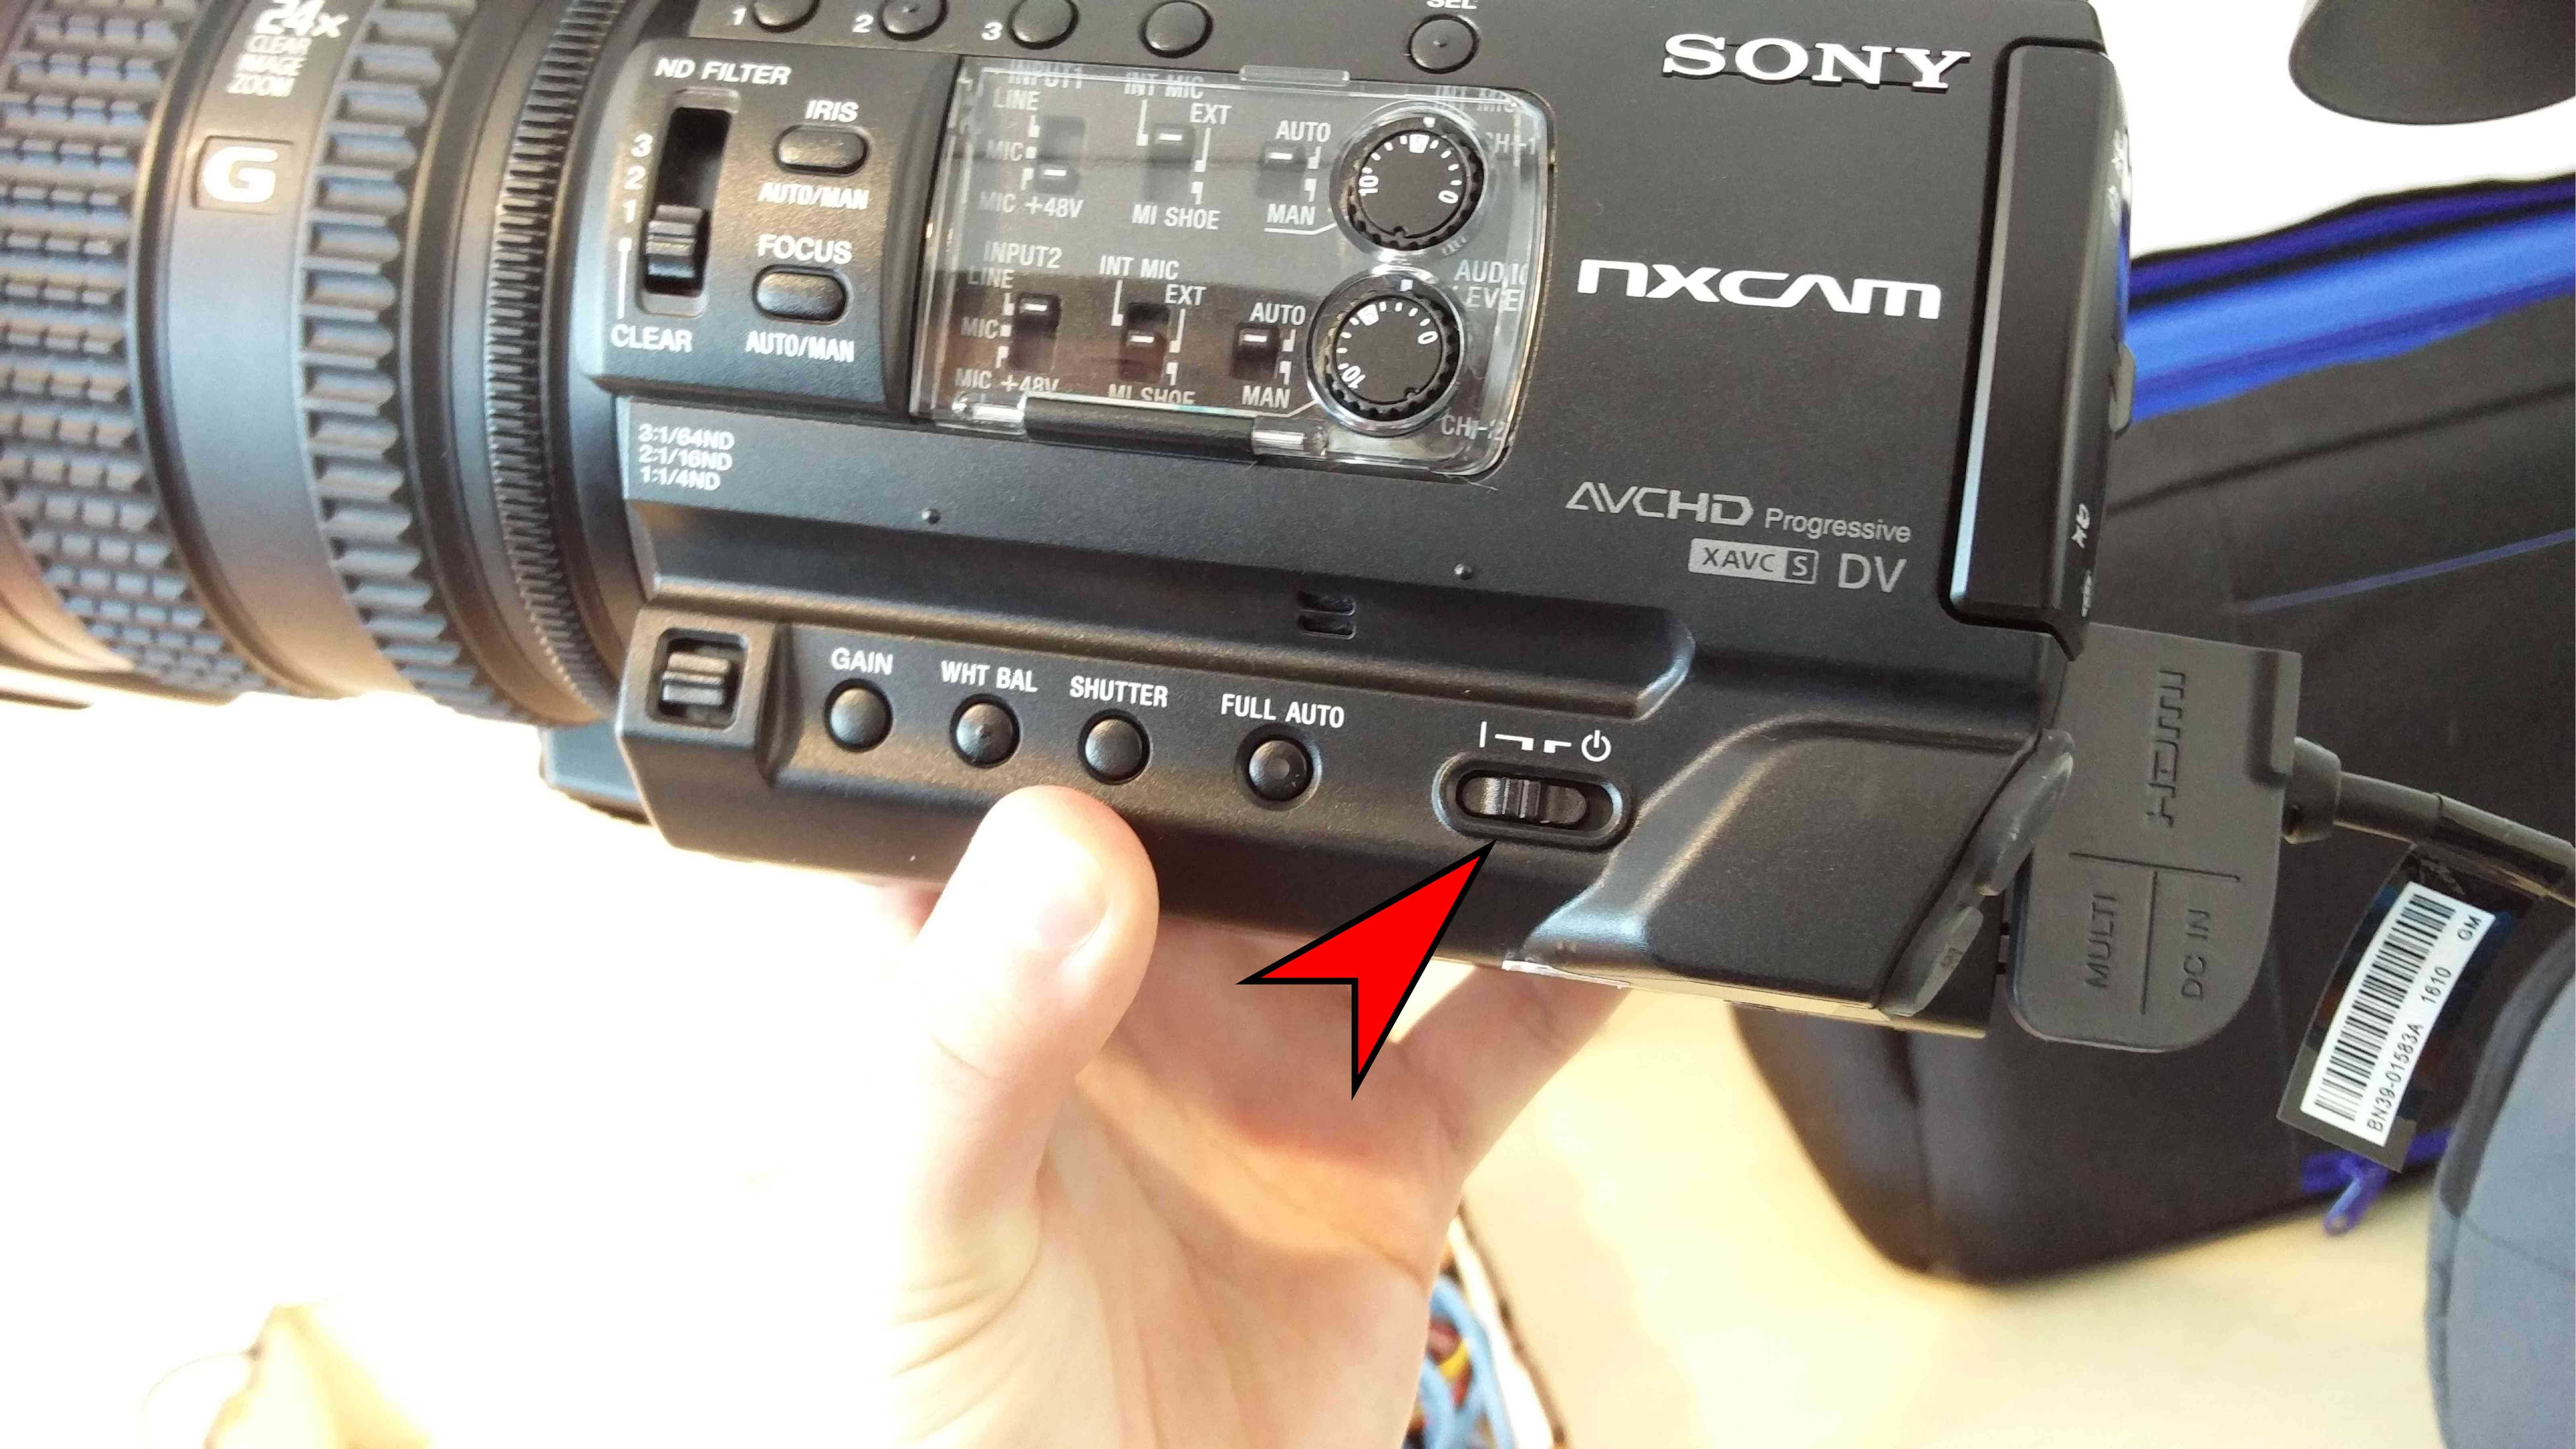
\includegraphics[width = 120mm]{Sony03.jpg}
\end{figure}

\subsubsection{Factory default settings}
Does the camera ask for a time and date? Then you can skip this section, as it already is on factory default settings.
Does the camera NOT ask for a time and date? Then we have to reset things.

First we reset all but the picture profile settings to factory default:
Menu $\rightarrow$ ``Others'' (three drawers icon) $\rightarrow$ Initialize $\rightarrow$ OK.

Now we set date/time. Not important. Just click the SET button a few times to get through this.

Then we reset picture profile 4 (the default picture profile) to factory default:
Menu $\rightarrow$ Camera set (camera icon) $\rightarrow$ Picture profile $\rightarrow$ PP4 $\rightarrow$ Setting $\rightarrow$ Reset $\rightarrow$ Yes.

\subsubsection{Audio settings}
The audio settings can only be done through the hardware switches on the camera.
Make sure to set the switches to the correct positions, as these directly affect the availability of audio on the recordings and live streams. Wrong settings means no audio!
If unsure, verify with the image below.

\begin{tabular}{| l || l | l | l | l |}
\hline
Input & Left switch & Middle switch & Right switch & dial \\
\hline
Input1 & BOTTOM (Mic 48V) & MIDDLE (EXT MIC) & BOTTOM (MANUAL) & 5 \\
Input2 & BOTTOM (Mic 48V) & TOP (INT MIC) & BOTTOM (MANUAL) & 5 \\
\hline
\end{tabular}

\begin{figure}[H]
  \centering
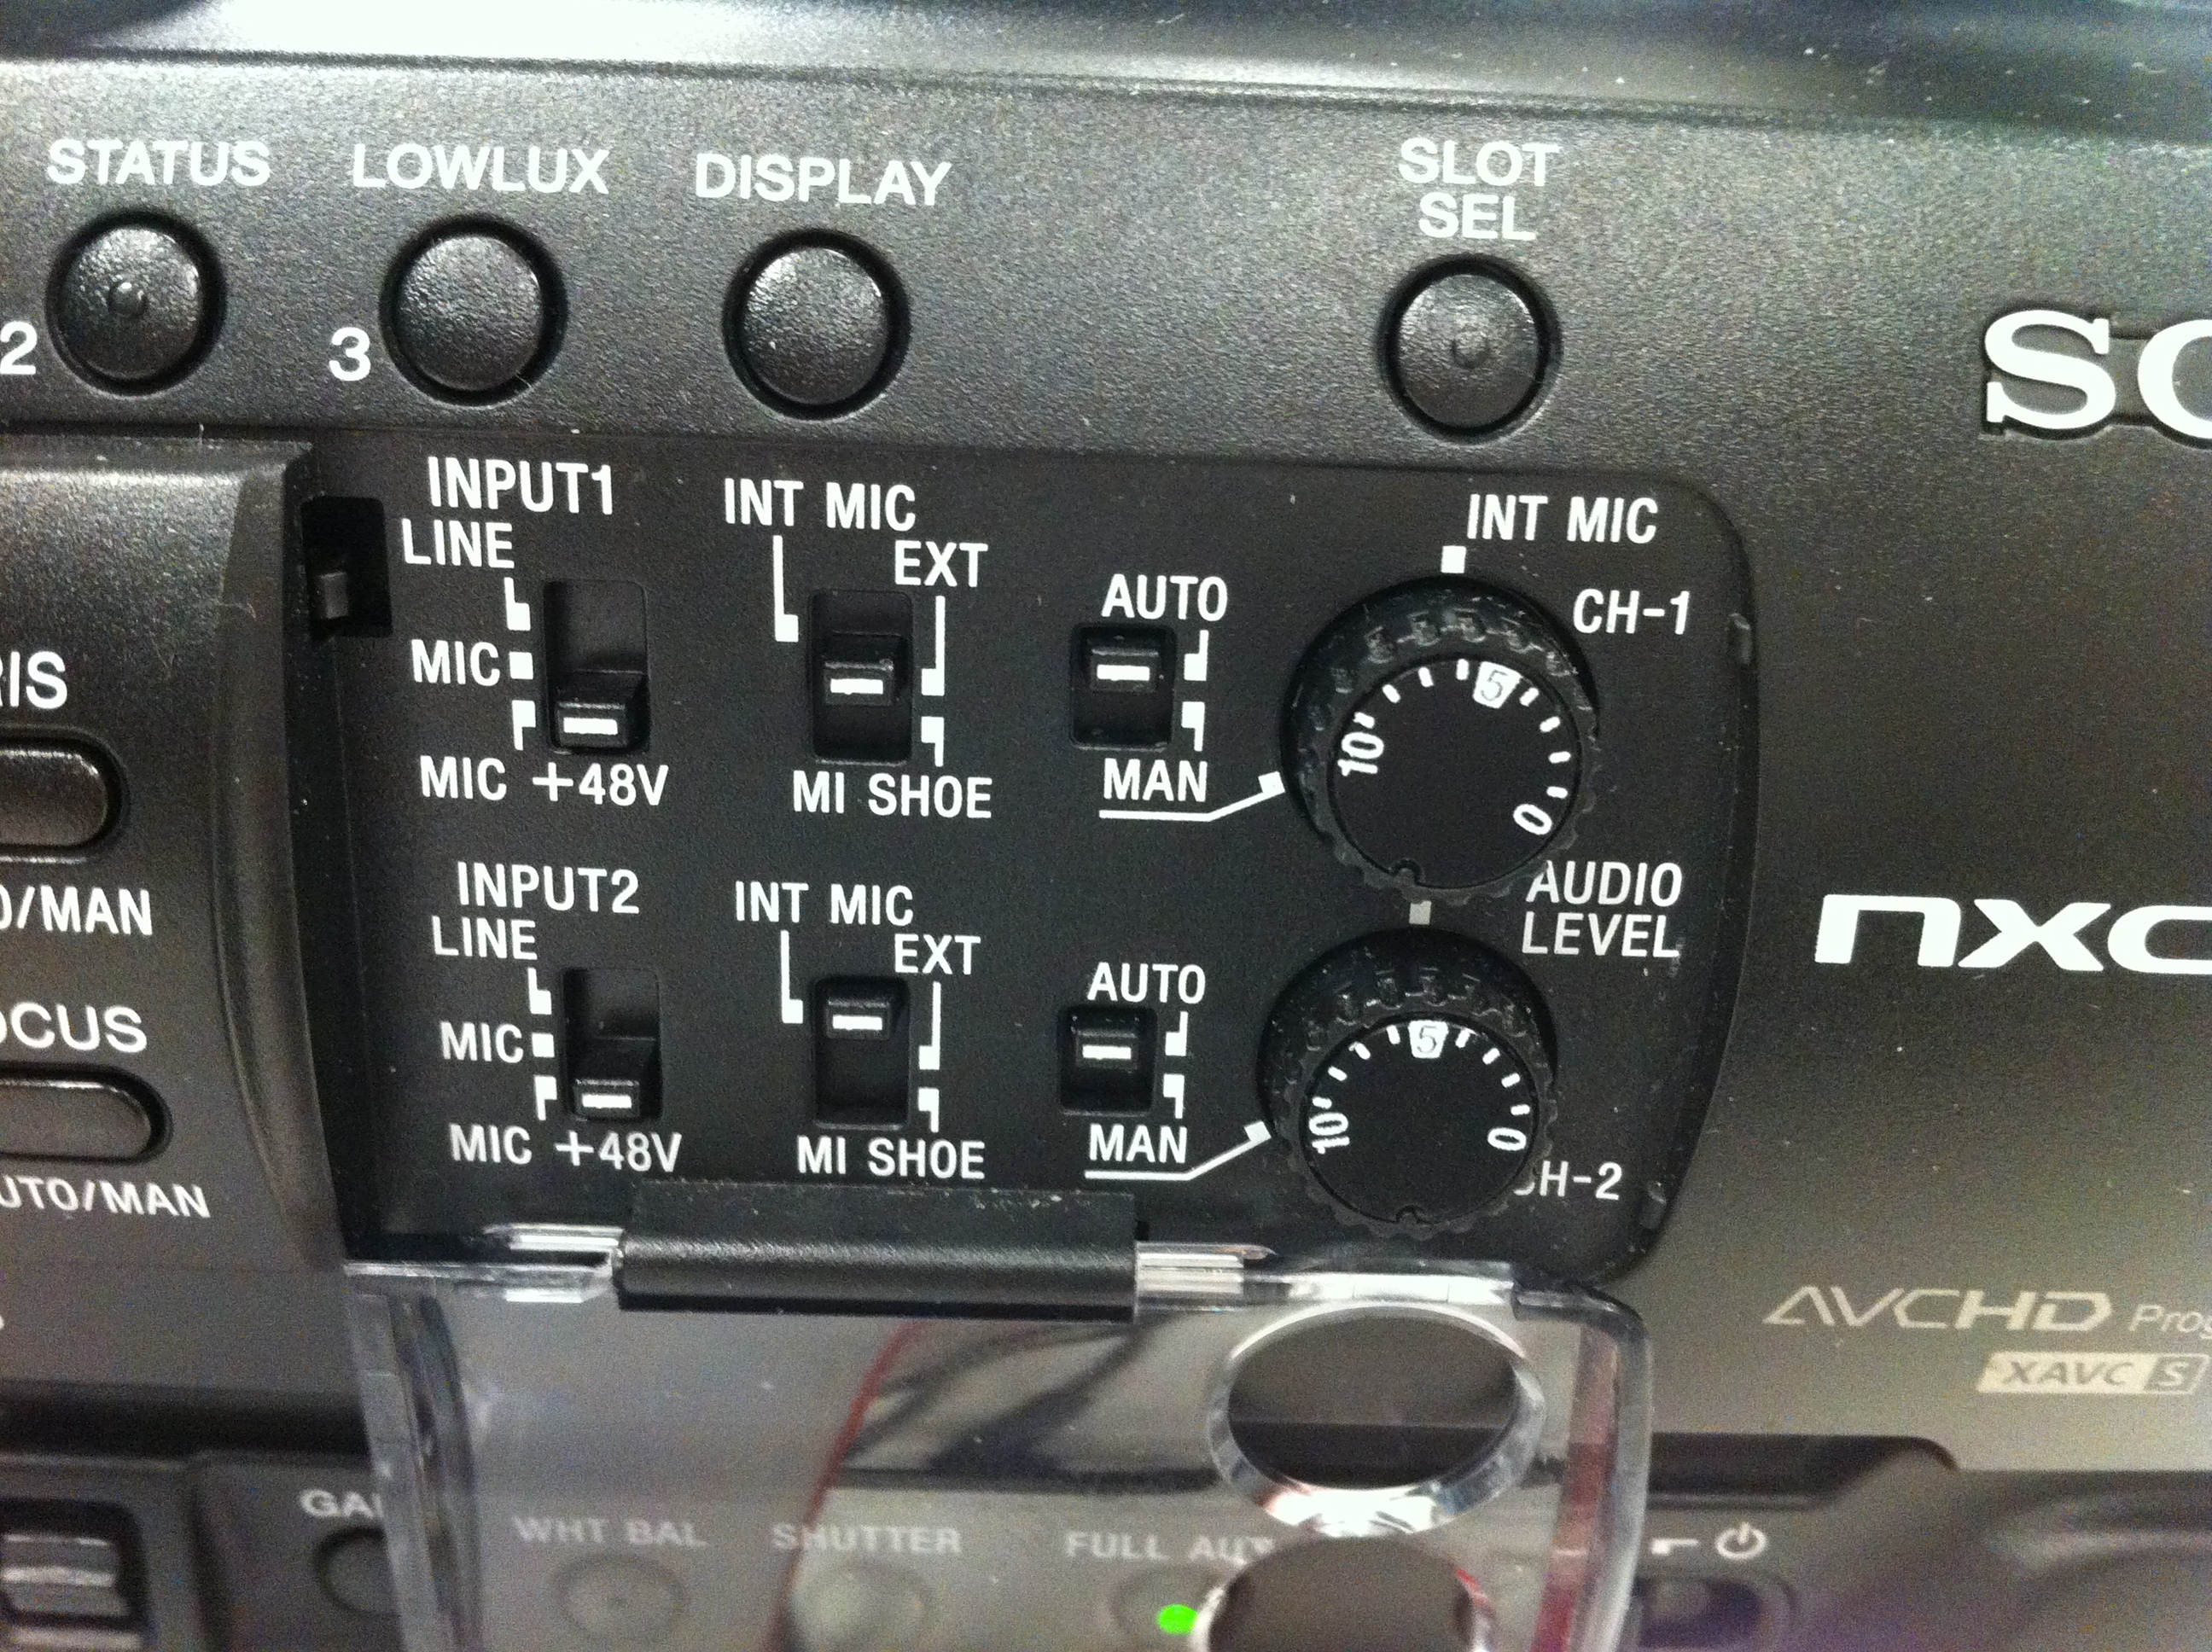
\includegraphics[width = 120mm]{sony_audio_settings.jpg}
\end{figure}

\subsubsection{Audio levels}

To configure the audio levels, use the following procedure for small rooms:
\begin{itemize}
  \item Set the levels to 5 for both channels;
  \item For the internal camera microphone (channel 2, small rooms) talk loud near the camera and make sure the levels don't go over the end (using the dial);
  \item For channel 1 (speaker microphone) yell while wearing the microphone and make sure the levels don't go over the end (using the dial);
\end{itemize}

For the other (large, XXL) rooms:

\begin{itemize}
  \item Set the levels to 5 for both channels;
  \item For the speaker microphone yell while wearing the microphone and make sure the levels don't go over the end, adjusting from the mixing console;
  \item For all the other microphones, talk moderately loudly while adjusting the microphones, making sure that they don't go over the top;
  \item Adjust the overall volume for the room to be audible as much as possible without creating feedback;
  \item Additionally test for feedback while moving with the microphone around the PA system in the room and adjust accordingly.
\end{itemize}

\subsubsection{Video output configuration}
The video configuration will be done through the on-screen display.

Set up like this:

Menu $\rightarrow$ 2nd icon (two arrows) $\rightarrow$ Video out $\rightarrow$ HDMI $\rightarrow$ 1080p.
\begin{figure}[H]
  \centering
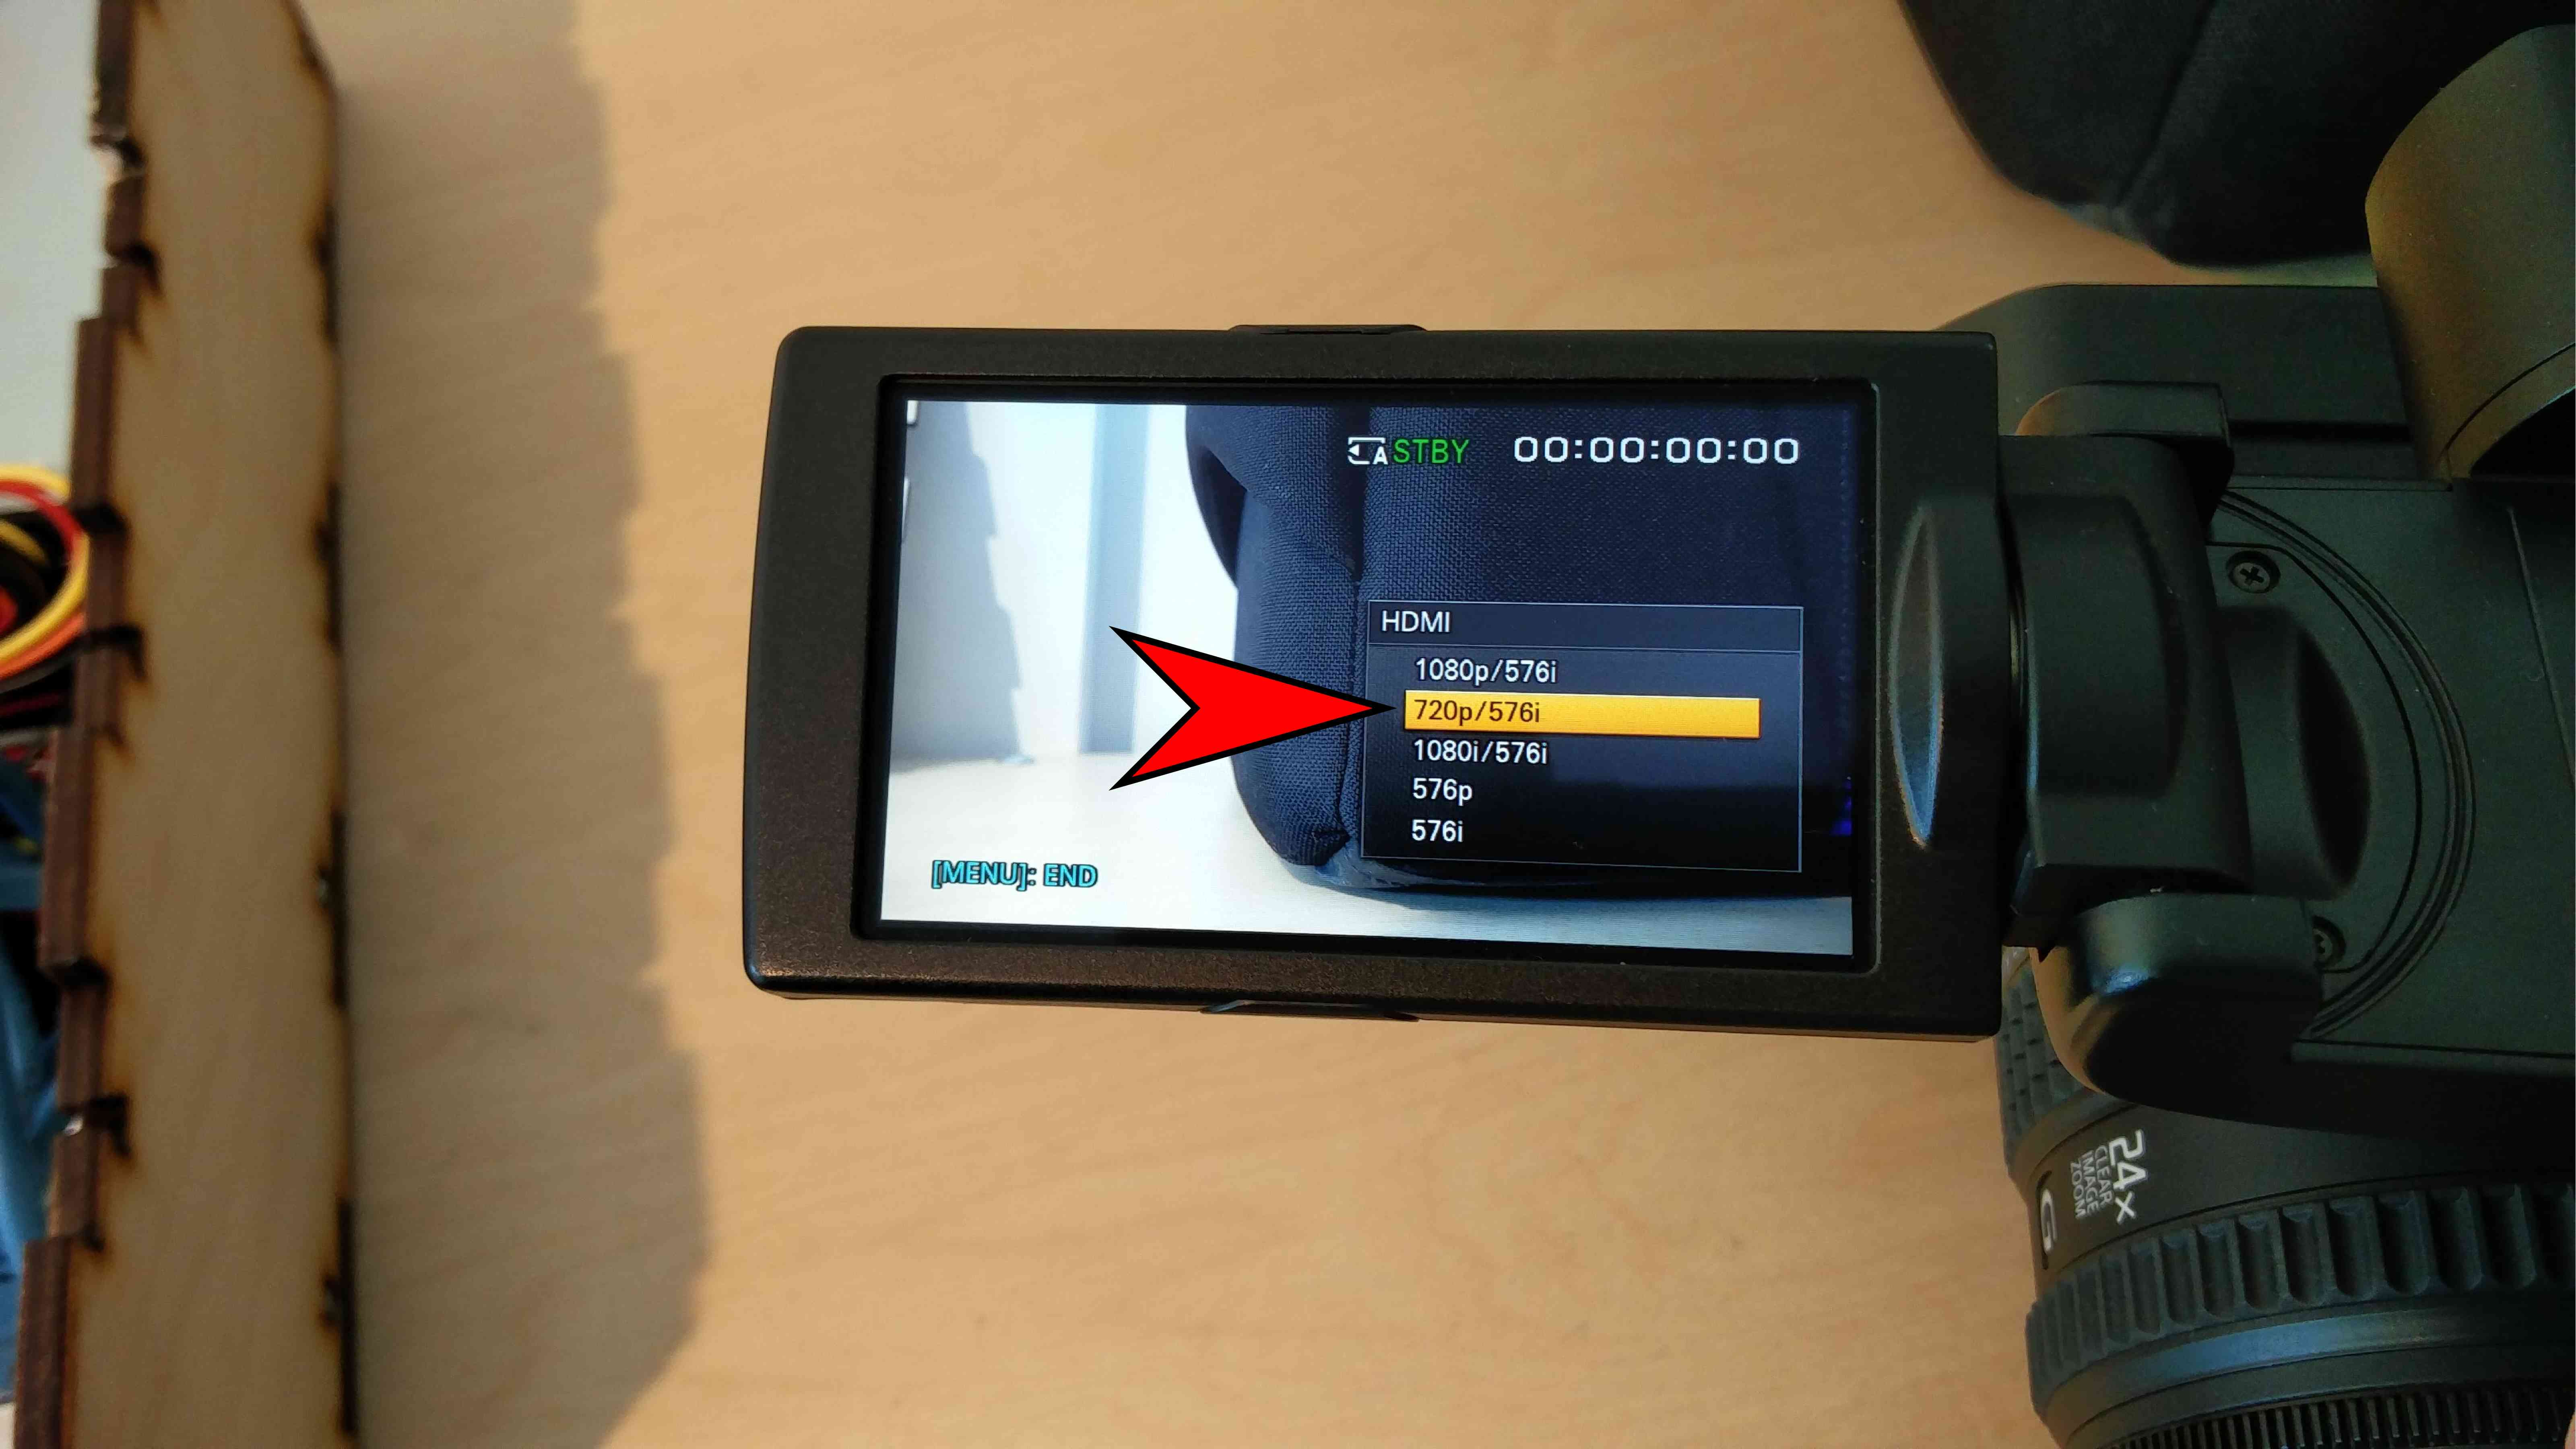
\includegraphics[width = 120mm]{Sony05.jpg}
\end{figure}

The resolution information displayed on the OSD relates to recording to the SD card, which we do not use. \emph{Ignore this text}, as the video output config is completely separate from the recording setting on this model.
\begin{figure}[H]
  \centering
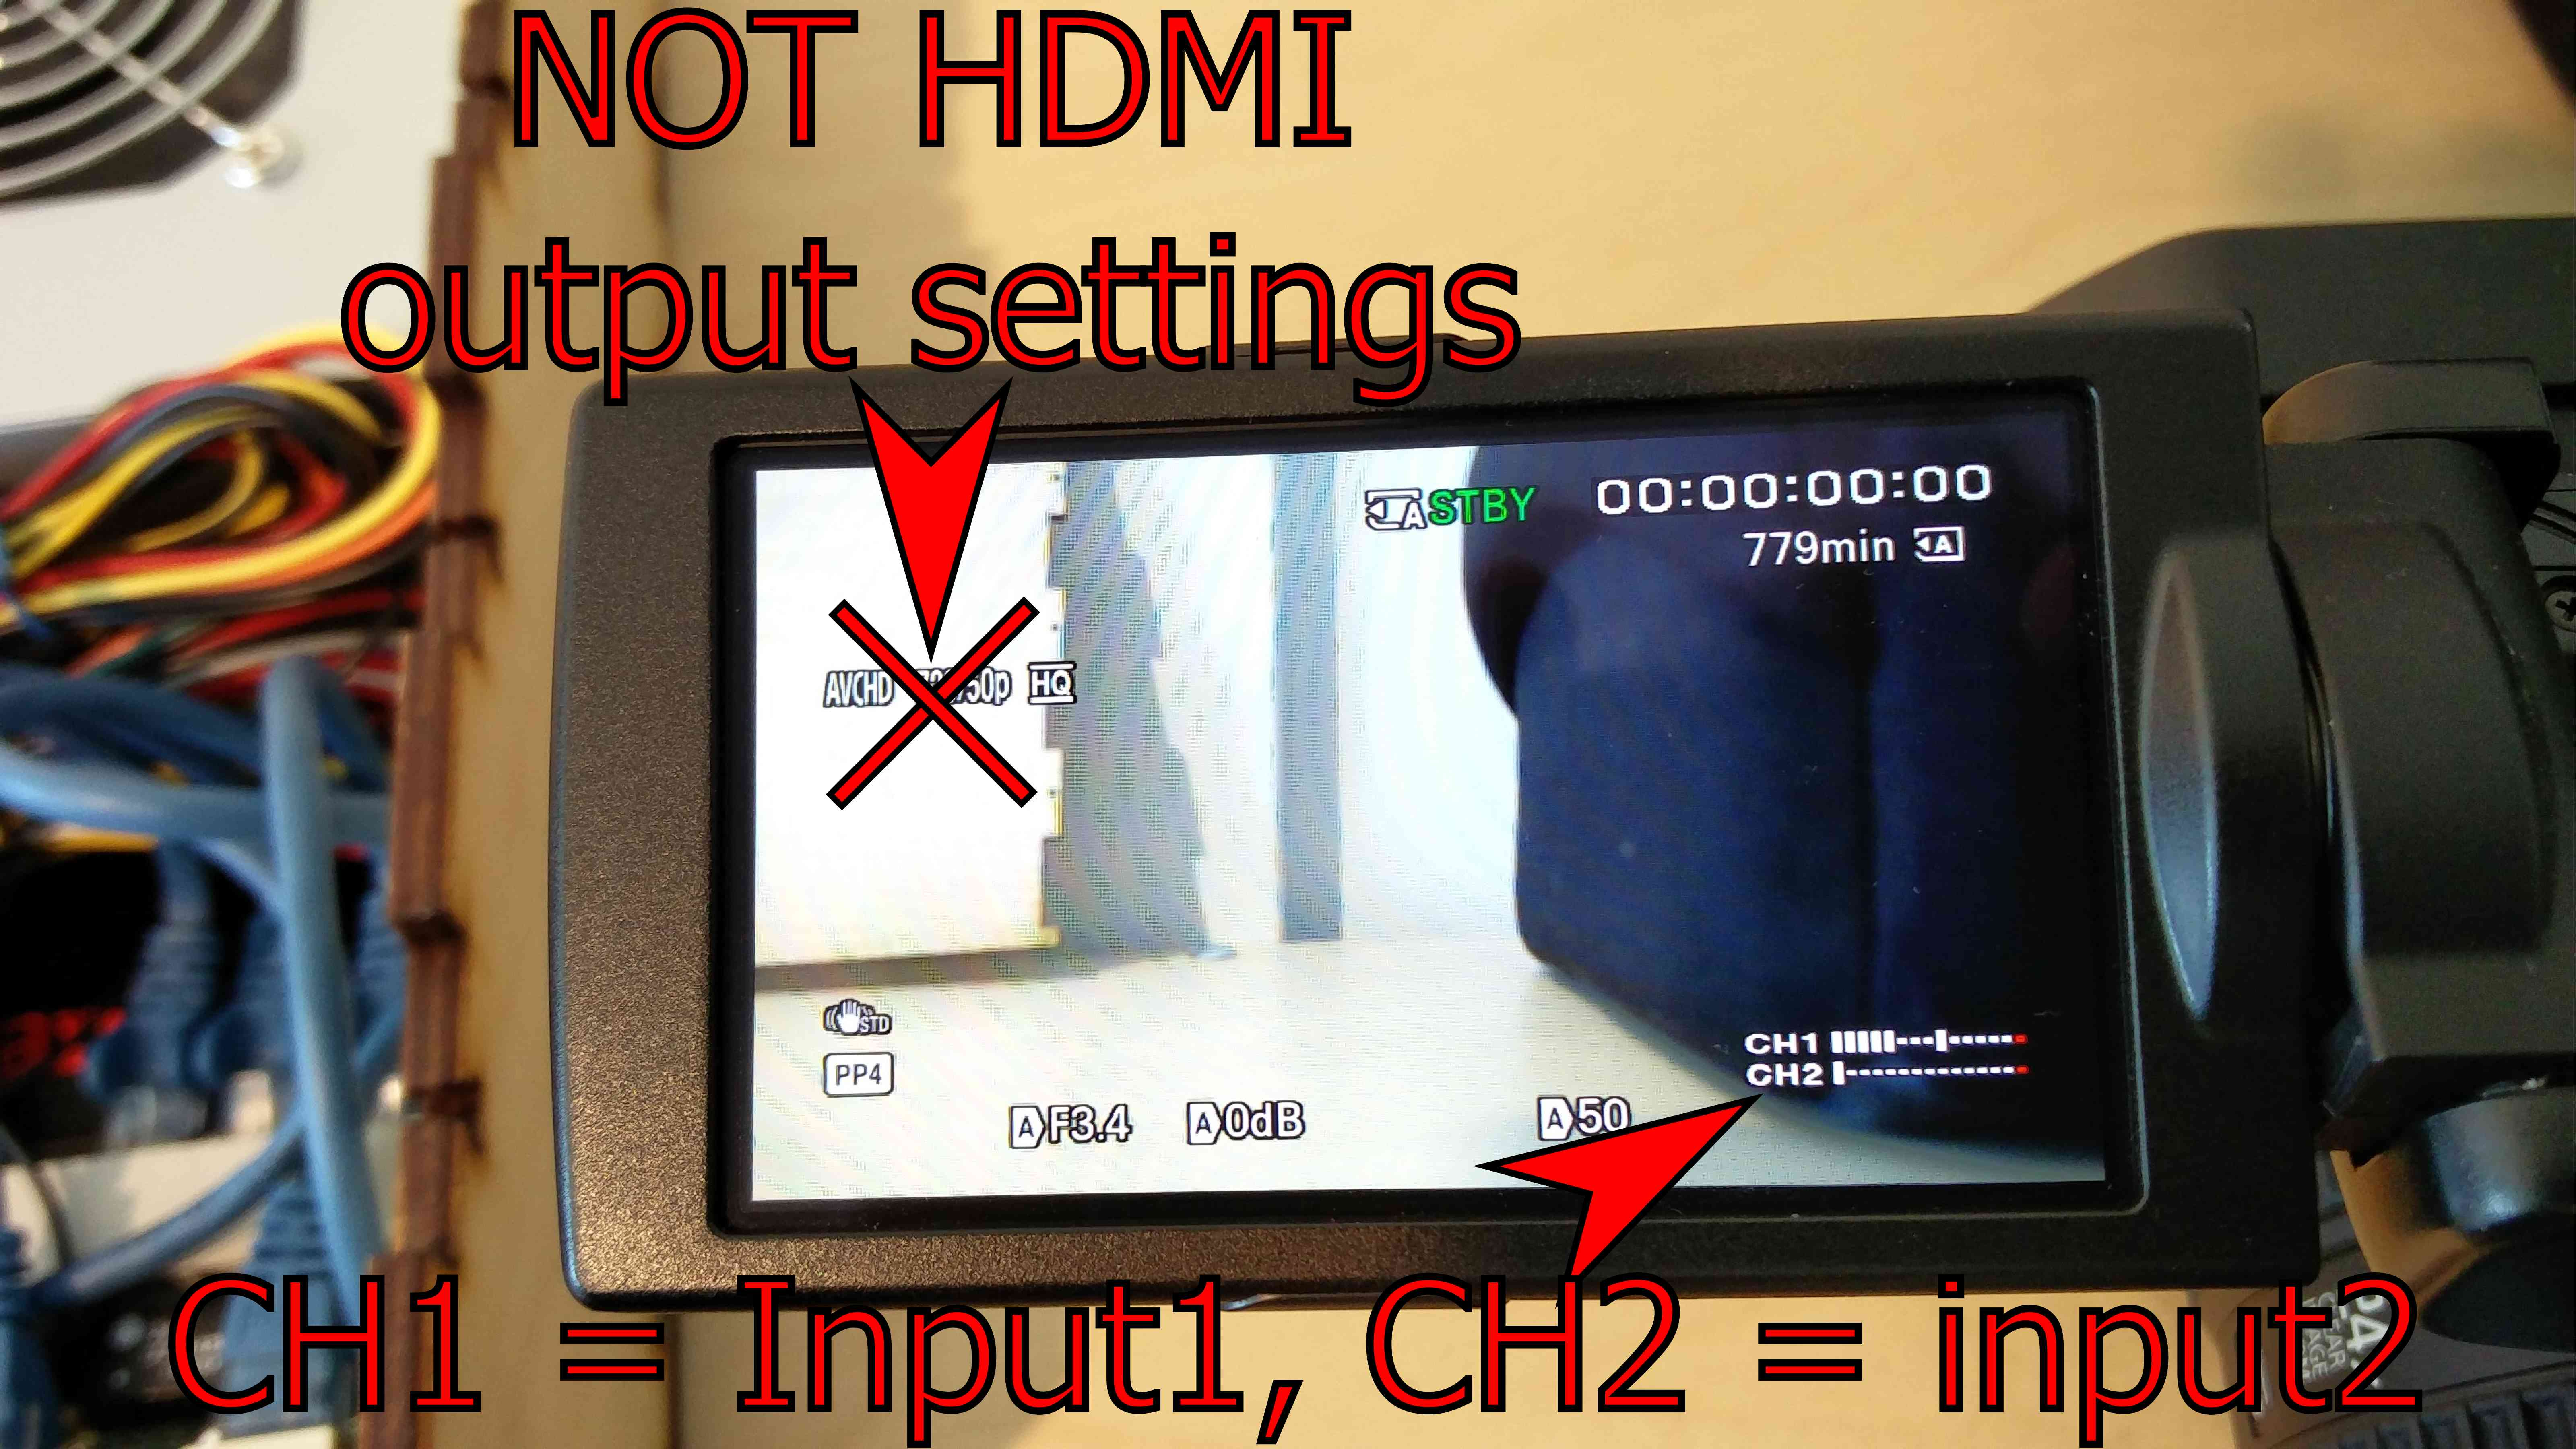
\includegraphics[width = 120mm]{Sony06.jpg}
\end{figure}

For rooms with low light conditions only, press button 3 (LOWLUX) to have the camera auto adapt to low light levels. A candle icon appears in the bottom right corner of the OSD screen.

\subsubsection{Remove the lens cover}
\emph{Do not forget to remove the lens cover.} Store it in the camera bag for safe keeping.

\begin{figure}[H]
  \centering
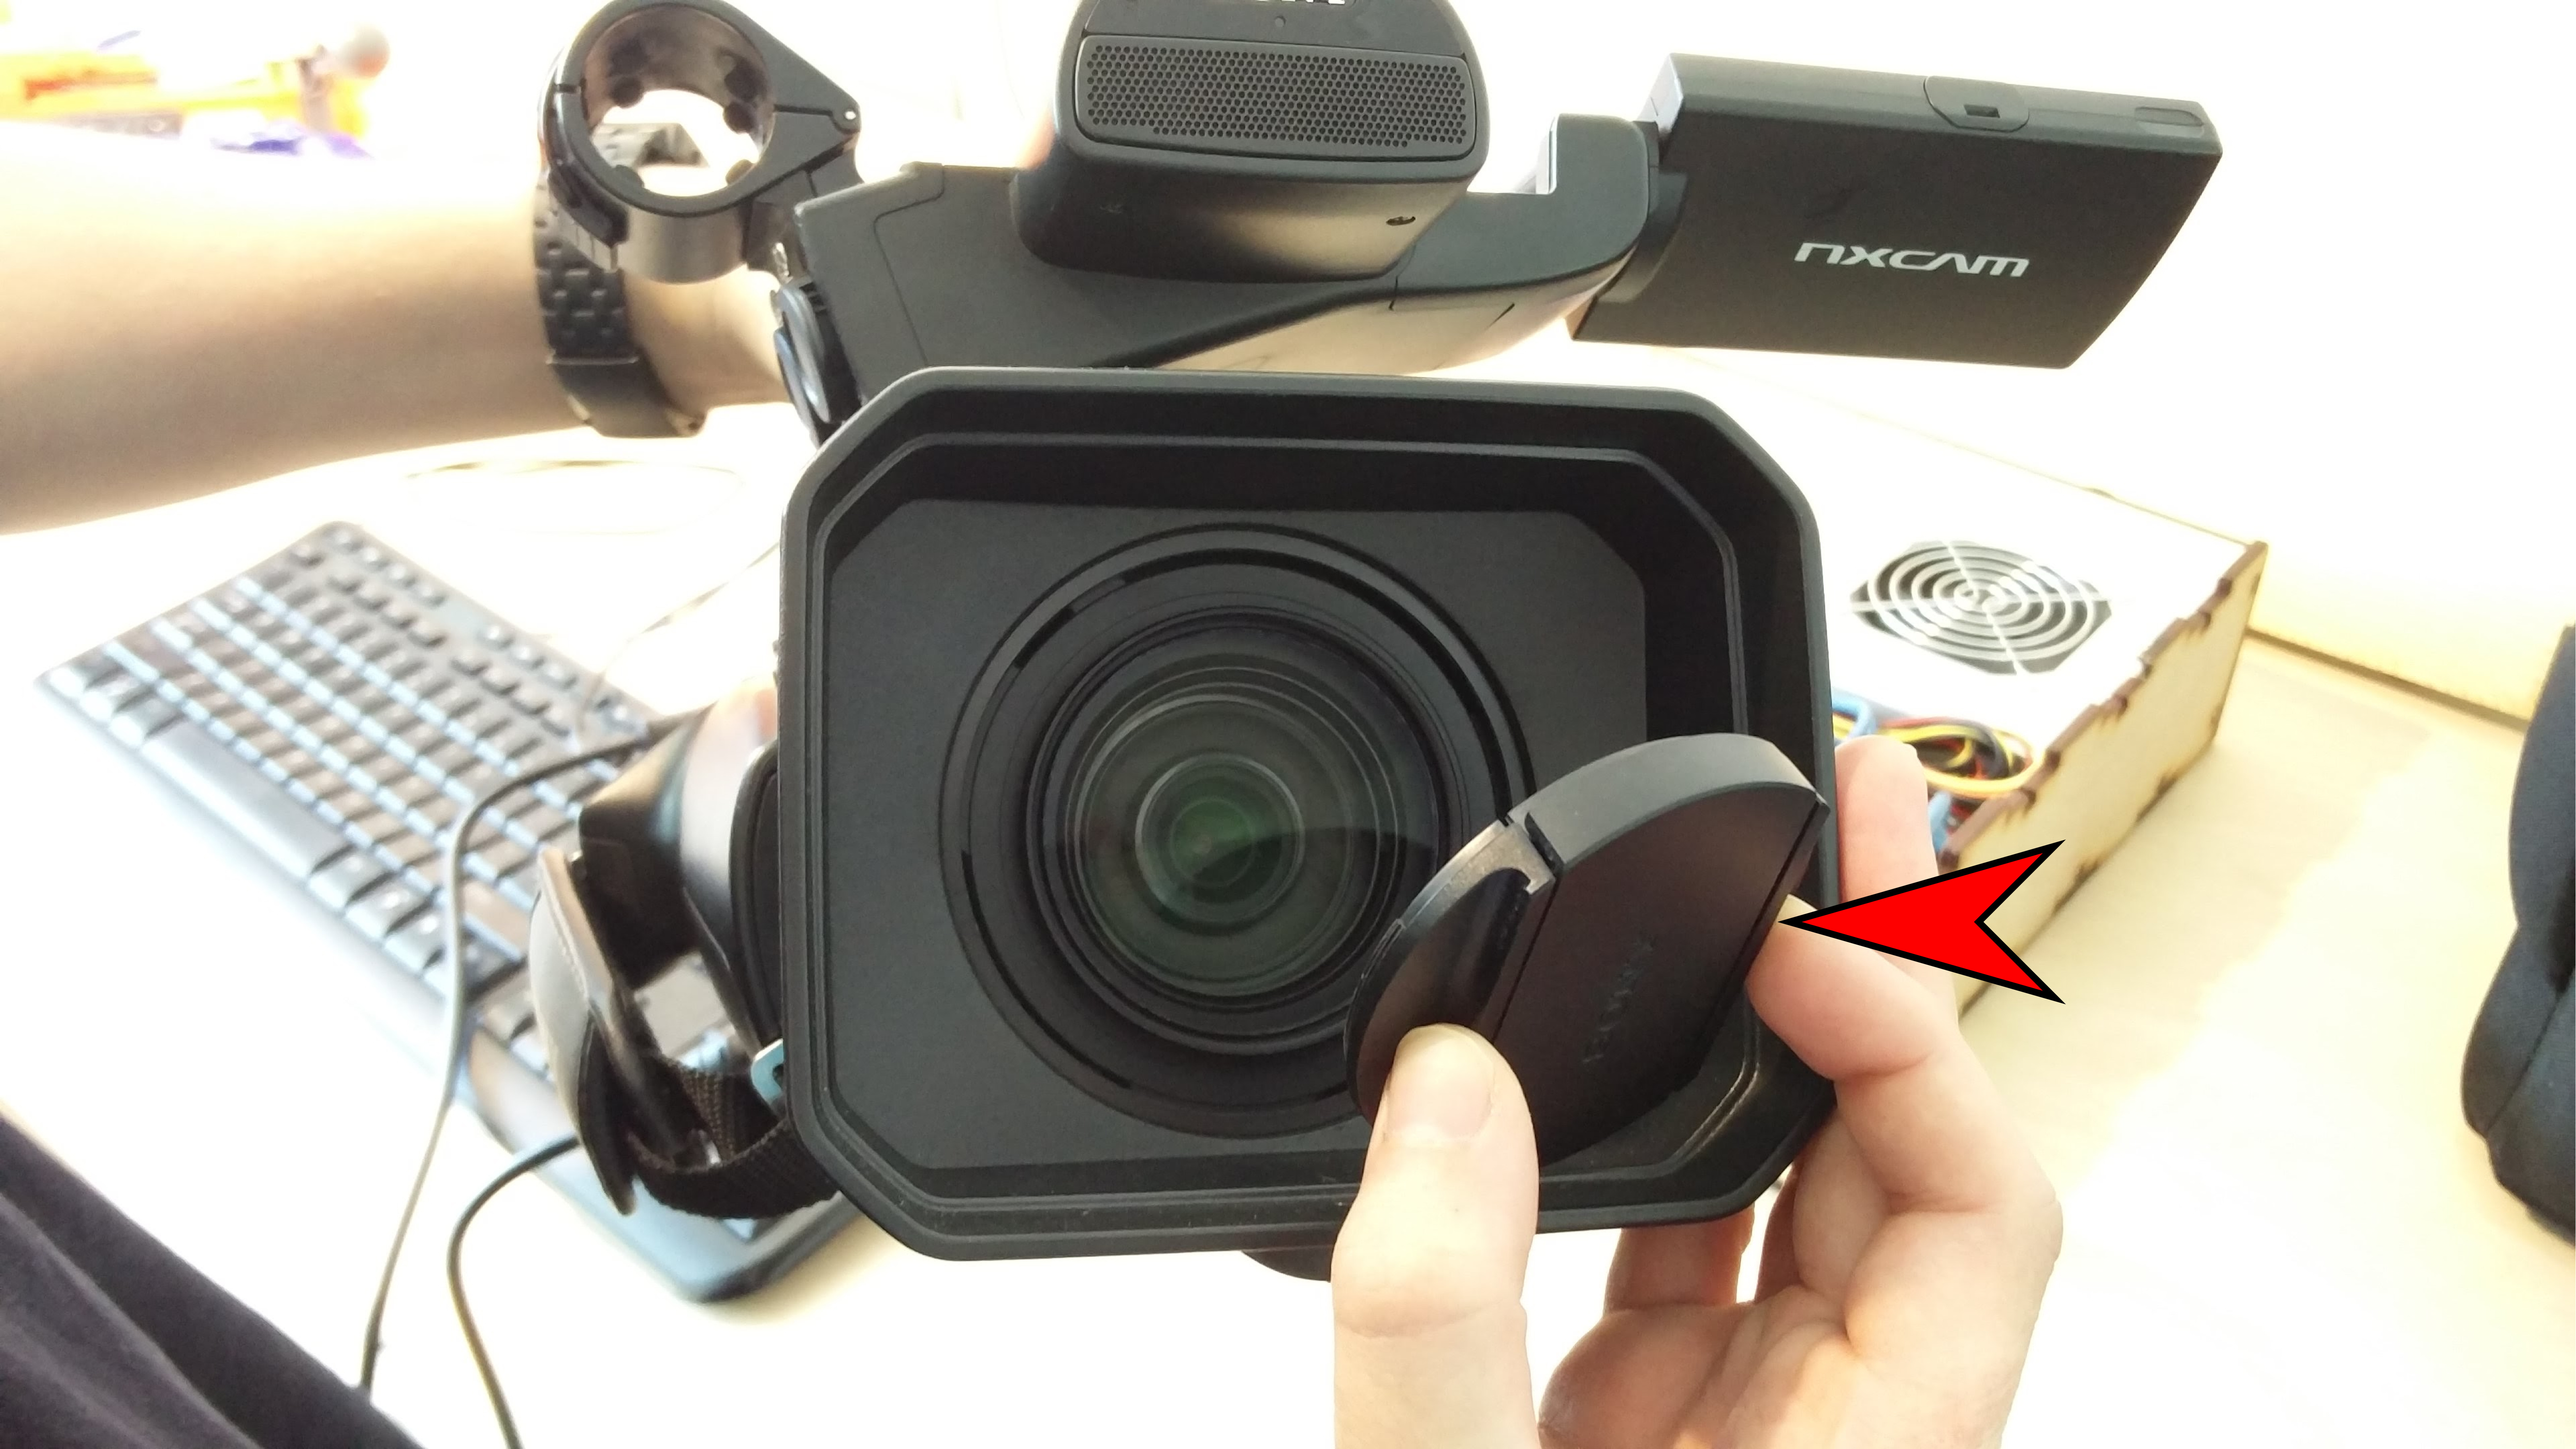
\includegraphics[width = 120mm]{Sony07.jpg}
\end{figure}

\subsubsection{Checklist}
Please check the following before leaving:
\begin{itemize}
  \item Does CH1 on the camera display spike when you tap the (powered on) wireless speaker microphone?
  \item Does CH2 on the camera display spike when you tap the camera itself with your fingers?
  \item Turn off the wireless speaker microphone before leaving to conserve battery power for during the day.
  \item Do both video boxes say mode 1080p50 on the LCD display?
  \item Does the camera video box display the camera image on the LCD display?
\end{itemize}

If any of these do not work, re-check your connections and settings. Still no luck? Contract VOC!

\subsubsection{Contact control}
When you have finished setup of the room, please report to VOC for a full test.
They will let you know what rooms still need attention.

\section{During the event}
It is expected of the devroom video volunteers that they keep an eye on the following, in order of importance:
\begin{itemize}
  \item The wireless speaker mic is on during talks
  \item The wireless speaker mic is worn correctly (see below)
  \item The audio volume is not too low or too high (clipping is bad!)
  \item The camera is aimed at the speaker, \emph{not} the projection screen (the projection screen is captured separately!)
  \item None of the video equipment is stolen or tampered with
  \item The video boxes/laptops are turned on and have OK network status.
\end{itemize}
The main task is ensuring audio quality. Video quality, while important, is only a secondary concern. A recording without video is still usable, but a recording without audio is completely useless.

The correct way to wear a lapel mic is as follows:
\begin{itemize}
  \item The microphone is attached at speaker's clothes near the neck, under the chin (centrally);
  \item There are no necklaces or lanyards that would touch it during the talk;
  \item There are no scarves or similar that cover the microphone or will touch it;
  \item The microphone is attached to the topmost layer of clothes (so there's nothing above it that would touch it);
  \item If there is no place where the microphone can be attached, a lanyard can be used for this purpose, on top of all the clothing of the speaker;
  \item The microphone receiver is attached to the belt of the speaker. If not possible, it's attached on top of a pocket;
  \item If the speaker has neither a belt nor pockets, he/she can hold the receiver in hand, or worst case scenario, it can be attached with duct tape to the waist (with a full loop around the waist) \emph{(this is a joke, do not duct-tape speakers)}
  \item The speaker is notified that if he's not facing in the direction of the microphone (e.g. not looking straight) the audio will be less audible.
\end{itemize}

Video team members will be both monitoring remotely as well as visiting rooms with problems. If you have questions, concerns or problems and there is no video team member nearby, contact them
%through the \texttt{\#video:fosdem.org} channel on Matrix https://chat.fosdem.org/\#/room/\#video:fosdem.org or
in \texttt{FOSDEM Video}. If your video box shows issues on the LCD, most likely somebody is already on their way to you. When communicating with video team members, please mention the \emph{room number} as opposed to the devroom name. Devrooms move around, room numbers stay constant.

\section{System infrastructure overview}

This section explains how the video streaming and recording works in general
for FOSDEM, to use as a helper to understanding the system and dealing with
issues.

The system's code and recipes for deployment are available in FOSDEM's GitHub
repo \texttt{infrastructure}, in the \texttt{ansible} subdirectory.

This is a general schema of the setup:

\begin{figure}[H]
  \begin{sideways}
  \centering
  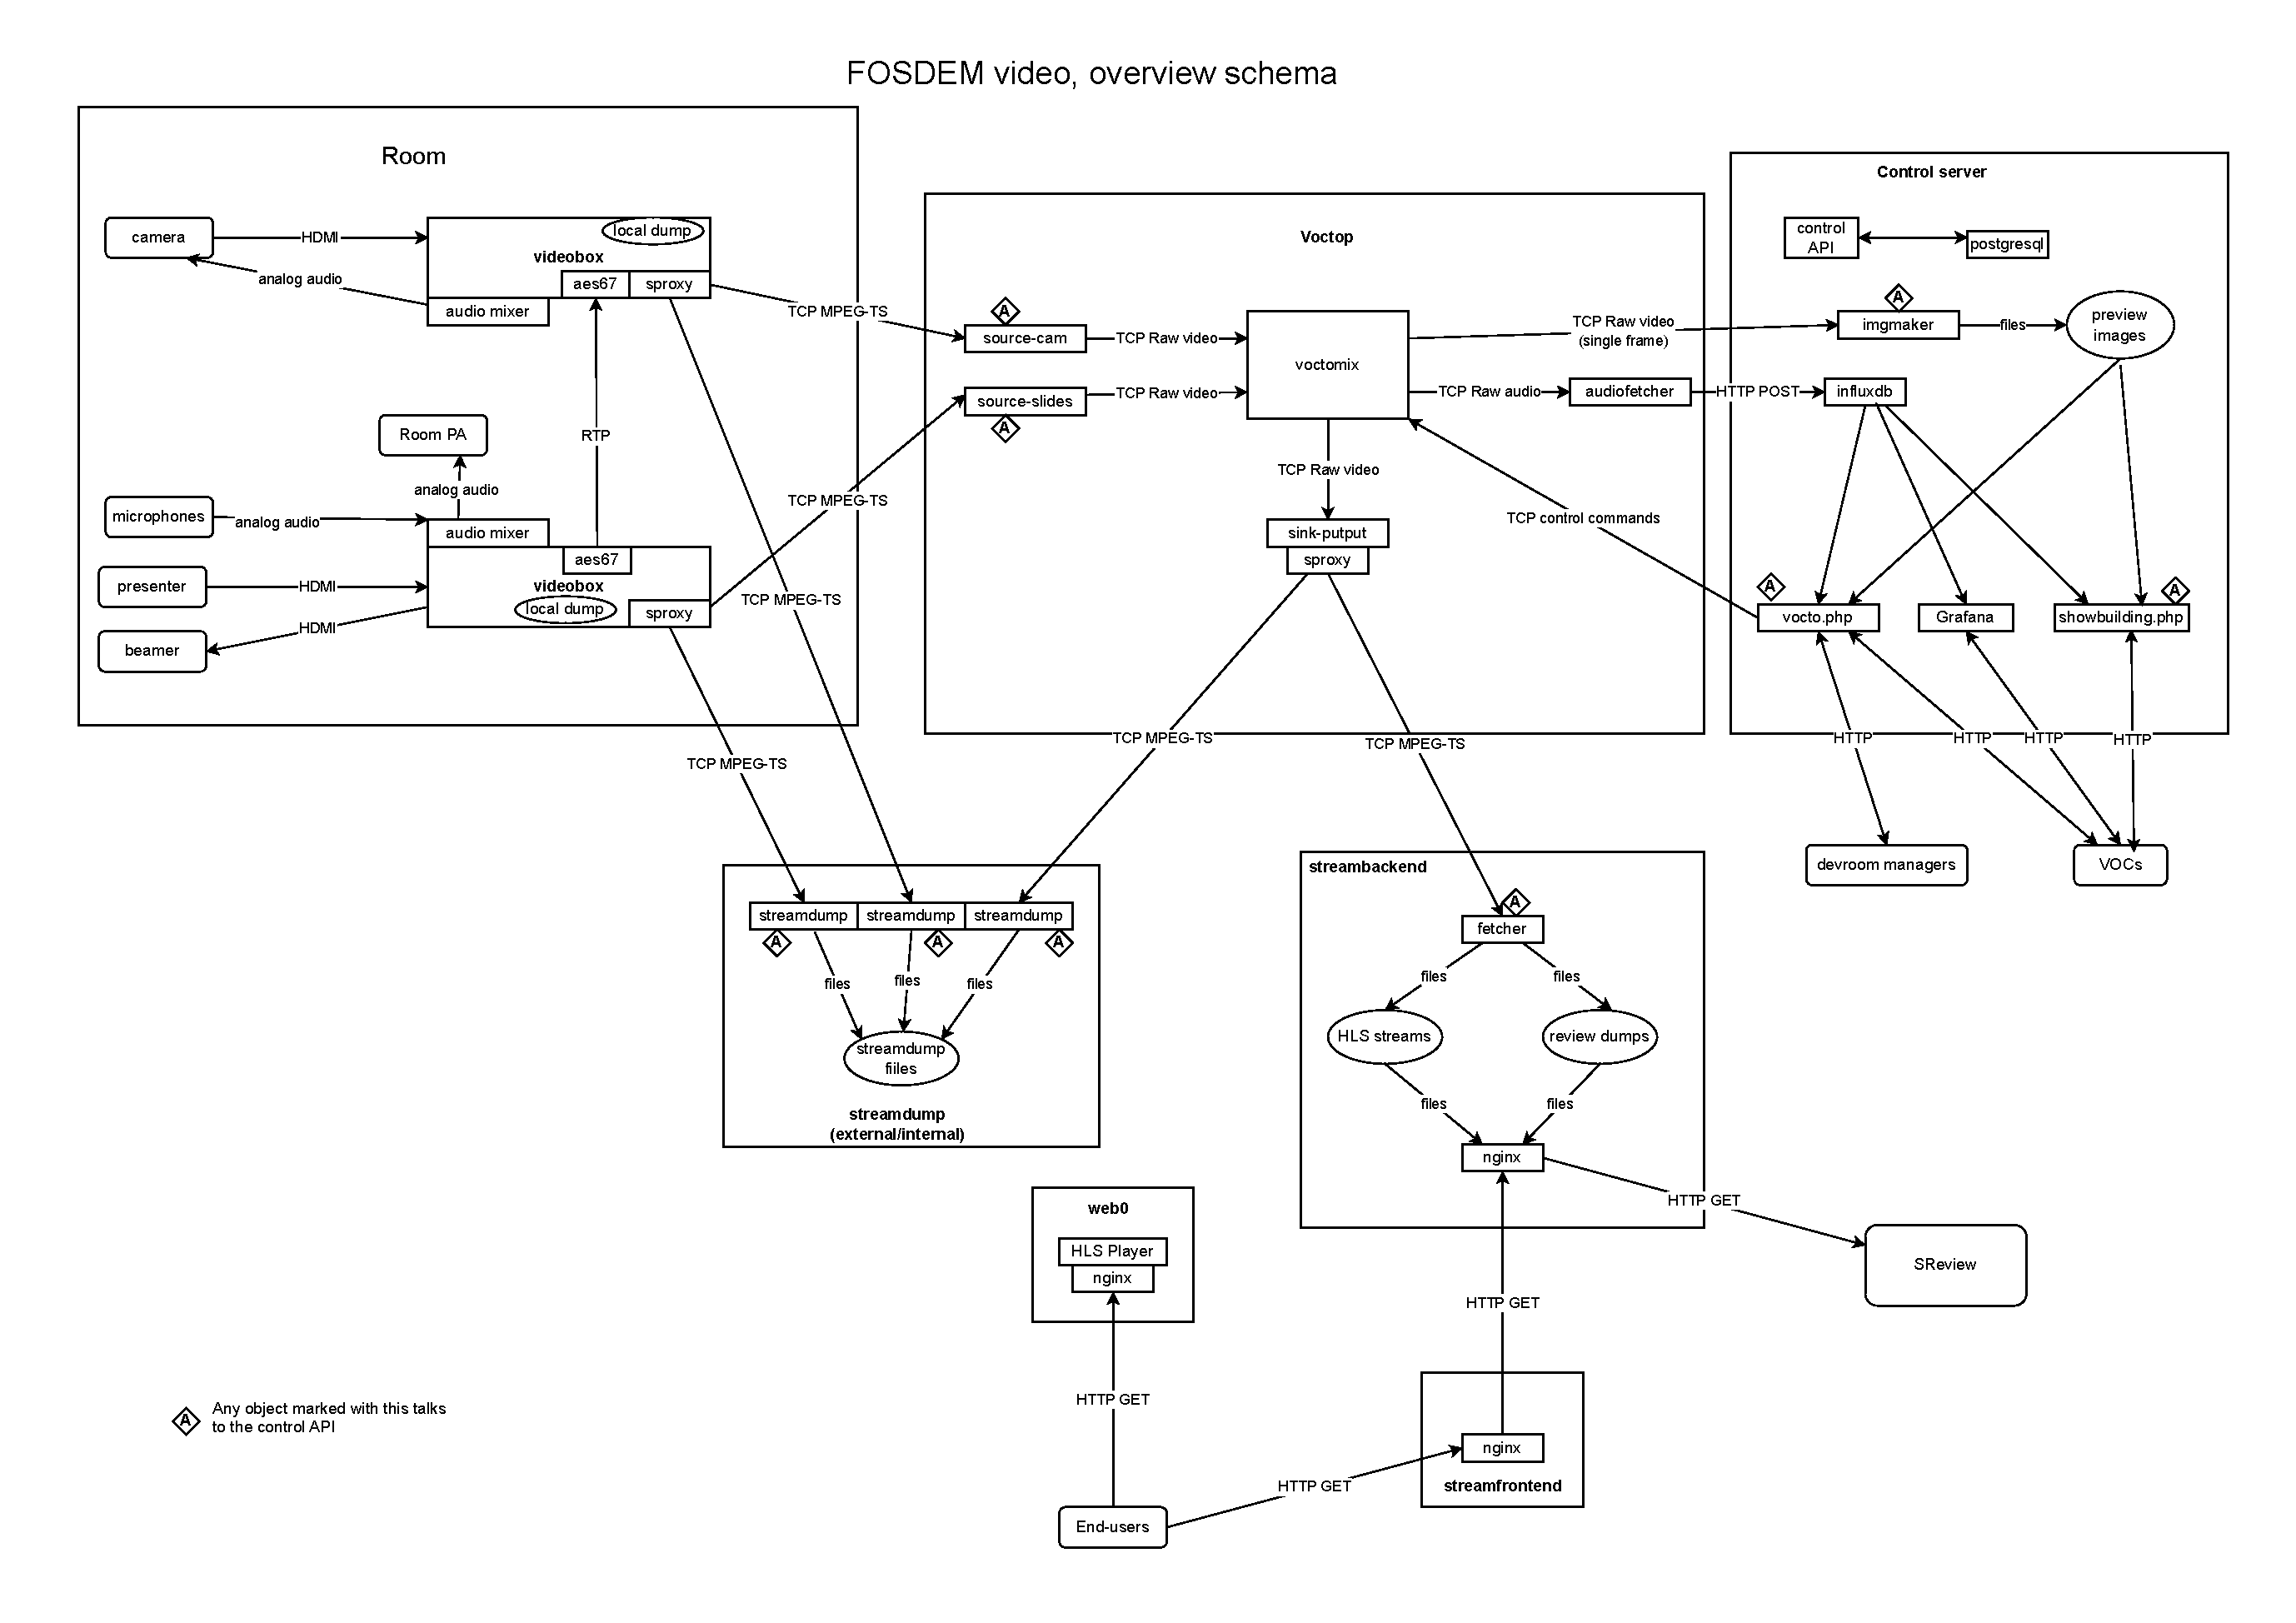
\includegraphics[width = 200mm]{../../graph/overview.pdf}
  \end{sideways}
\end{figure}


Below is a list of components (some software, some whole-system) that are the pieces of the whole thing.

\subsection{sproxy}

\texttt{sproxy} is a small piece of software available in https://github.com/FOSDEM/sproxy and FOSDEM's Debian package repository. It's written in C and its role is to receive a stream of bytes on \texttt{stdin} in a ring-buffer and provide the following TCP endpoints (up to 32) to clients:

\begin{itemize}
  \item Port 8899 - this provides the stream from the current point onward. This is used for normal video clients that want to access the stream as it's being pushed at the moment;
  \item Port 8898 - this provides the stream with half of what's currently in the buffer, to allow clients to quickly start displaying the stream. This is used mostly for debug purposes, as it just makes it faster to find a keyframe;
  \item Port 80 - this provides the stream from the current point onward, after it receives some HTTP headers. This was implemented for compatibility with some streaming devices for the 2020 edition.
\end{itemize}

The main use of \texttt{sproxy} is to allow multiple clients to access a
MPEG-TS encapsulated video (H.264, AAC) in real time without the need of any
previous setup. MPEG-TS allows this, as it's not relevant when in the stream
the client starts reading, as the encapsulation is self-synchronizing.

\texttt{sproxy} is the successor of multicast UDP running over the network, as
that proved to create hard to debug problems with even moderate packet loss
(which TCP doesn't have).

\subsection{video-box}

Implemented in role \texttt{video-box}.

The \texttt{video-box} is in general a capture device that provides \texttt{sproxy} interface from its video and audio capture, plus some monitoring functions.

Its hardware consists of a laptop and a box that connects to the laptop via a short USB 3 USB-C cable. In the box you can find:

\begin{itemize}
  \item HDMI capture device, based on the MacroSilicon MS2131 chip. The two HDMI ports on the box are connected to it;
  \item A 4-port USB network controller that also acts as switch;
  \item An USB hub (dock), that is used to connect both the above devices to the laptop.
\end{itemize}

The laptop is used to:

\begin{itemize}
  \item Capture video and audio from the HDMI capture device, synchronize them (with a fixed offset) and encode them using the hardware acceleration available in the CPU/GPU;
  \item Present the captured video via \texttt{sproxy} to the network;
  \item Provide a preview of the video on the screen with a bar to show the sound levels (upper right);
  \item Provide status for the box and stream (upper left);
  \item Provide a terminal for debugging if needed (bottom left);
  \item Make a backup recording on its disk of the full stream for emergencies;
  \item Show the nice purple FOSDEM color as a background.
\end{itemize}

\subsection{video-voctop}

Implemented in role \texttt{video-voctop}.

The \texttt{voctop} is the video mixer that fetches the streams for the camera
and presenter from a room, and provides the ``finished'' video stream to the
streaming and recording infrastructure. The finished stream is again presented
via \texttt{sproxy}.

The mixing is done using \texttt{voctomix} (version 1). There are three sources
for \texttt{voctomix}:

\begin{itemize}
  \item \texttt{cam}, fetched from the box marked to be camera in the room;
  \item \texttt{grabber}, fetched from the box marked to be slides/presenter in the room;
  \item \texttt{background} that contains artwork/the year, and is the thing most forgotten to be updated every year.
\end{itemize}

All streams are chewed and converted exactly to what voctomix requires (raw
video, 1080p, 25fps, SAR/DAR 1:1) and via a single \texttt{ffmpeg} instance a
MPEG-TS stream that contains video streams with 720p and 1080p is provided
via an \texttt{sproxy} instance.

The reason for mixing both video streams in the same MPEG-TS stream is that the
laptop runs out of memory bandwidth if another copy of the raw stream is taken
out of \texttt{voctomix}, and this also makes the preparation of the HLS
easier.

\texttt{voctomix} provides control via text protocol on port \texttt{9999}
which is used by the control server to switch the possible views/mixes of the
stream:

\begin{itemize}
  \item Full-screen camera;
  \item Full-screen presentation;
  \item Mix, large top-left presentation, small camera bottom right (the default);
  \item Mix, large top-left camera, small presentation bottom right;
\end{itemize}

Another piece of software, \texttt{audiofetcher} reads the audio stream, pushes its sound levels to an InfluxDB database on the control server, and also provides a Prometheus endpoint for the same.

\subsection{video-control-server}

Partially implemented in role \texttt{video-control-server}. Partially, because some of the stuff gets tweaked and updated on the running node before and during FOSDEM.

The following tasks are handled by the control server:

\begin{itemize}
  \item A database (with interface) of the mapping room$\rightarrow$voctop$\rightarrow$camerabox$\rightarrow$slidesbox. This is queried from the voctops and streambackend to know where to get the data for a particular room;
  \item An InfluxDB database with sound levels to which the \texttt{audiofetcher} from the voctop pushes data;
  \item A Grafana instance to plot the sound levels;
  \item A preview page with all rooms (selectable by building) showing camera/slides/mix and sound levels for every room (\texttt{showbuilding.php});
  \item A control interface for every room for changing the current video mix (\texttt{vocto.php}). It's authenticated with users/passwords provided to devroom managers;
  \item DHCP and DNS server for the video VLAN.
\end{itemize}

The majority of the traffic to the control server is the fetching of raw video
frames from the voctops, and amounts to a steady 300Mbps. This was the initial
reason to move this node on-site.

\subsection{video-streambackend}

Implemented in the role \texttt{video-streambackend}.

This is a (currently) single physical server outside of ULB that fetches all
mixed video streams from the voctops, and creates:

\begin{itemize}
  \item A HLS stream with two video (selectable) streams for viewing by end users;
  \item Half-hour dumps of video streams, to be processed by \texttt{sreview}
\end{itemize}

These are both created by using \texttt{ffmpeg}. The HLS stream is served via
\texttt{nginx} to the streamfrontends, and the dumps are served via either
\texttt{ssh}/\texttt{sshfs} or NFS to \texttt{sreview}.

\subsection{video-streamfrontend}

Implemented in the role \texttt{video-streamfrontend}.

This is a somewhat simple caching proxy implemented with \texttt{nginx} that
presents the video streams from the streambackend to end users.

\subsection{video-streamdump}

The \texttt{streamdump}'s role is to connect to all video-boxes and all
voctops, to fetch the video they provide to record it to be used for restore
for emergencies. There is usually one at ULB and one externally.

\subsection{HLS player}

\texttt{web0}'s role is to host the HLS player (implemented in JavaScript)
that end-users load to play the HLS stream with. It shows the video stream
for the relevant room and allows for selecting the video quality that
the users want so see.
 
\section{Historical notes}

Things done in the past that we moved away from:

\subsection{mod\_nginx\_rtmp}

The module is nice, but has serious limitations on multi-audio/video stream
processing, strange failures, and at some point didn't have any updates or
support. It was used to push from the voctops to the stereambackend. After its
removal, all video transfers became pull-based.

\subsection{multicast}

Sending MPEG-TS over UDP over multicast saved bandwidth due to the multiple
consumers of every stream. But packet loss in MPEG-TS was leading to subtle
issues in \texttt{ffmpeg}'s parsing and processing and needing the restart of
streams for issues that were hard to catch.

Experiments were done with flow control (didn't help) and reliable multicast
(the libraries didn't work, or at least Vasil was unable to make them), but
nothing came out of that, so \texttt{sproxy} was born.

\end{document}

